\documentclass{beamer}


% PACKAGES==========================================================================================
\usepackage{hyperref}
\usetheme[hideothersubsections]{PaloAlto}
\useinnertheme{rectangles}
\usecolortheme{beaver}
\usepackage[version=3]{mhchem}
\usepackage{caption}
\usepackage{textpos}
\usepackage{amsmath,esint}
\usepackage{etoolbox}
\usepackage{wrapfig}
\usepackage{multicol}
\usepackage[caption=false]{subfig}
%\usepackage[font=small,skip=0pt]{caption}


% SETTINGS==========================================================================================
\setbeamerfont{caption}{series=\normalfont,size=\fontsize{5}{5}}
\setbeamercolor{section in sidebar}{fg=black}
\setbeamercolor{section in sidebar shaded}{fg=lightgray}%section in sidebar.fg!40!bg}
%\setbeamercolor{section in sidebar}{fg=black}            %color of the active section
%\setbeamercolor{section in sidebar shaded}{fg=gray}     %color of the inactive section
\setbeamercolor{subsection in sidebar}{fg=darkred}         %color of the active subsection
\setbeamercolor{subsection in sidebar shaded}{fg=darkgray}  %color of the inactive subsection
\setbeamercolor{title in sidebar}{fg=black}              %color of the presentation title
%\setbeamercolor{author in sidebar}{fg=...}             %color of the author  
%\setbeamertemplate{section in toc shaded}[default][10]
 
 
\makeatletter
\patchcmd{\insertverticalnavigation}%
{\ifx\beamer@nav@css\beamer@hidetext{\usebeamertemplate{section in sidebar}}\else{\usebeamertemplate{section in sidebar shaded}}\fi}%
{{\usebeamertemplate{section in sidebar}}}{}{}
\makeatother 
 
 
\setbeamerfont{block body}{size=\tiny}
%\setbeamertemplate{blocks}[square][shadow=false]
\setbeamertemplate{blocks}[default]
\setbeamertemplate{bibliography item}[text]
\setlength{\parindent}{0pt}
\setbeamertemplate{caption}[numbered]


\defbeamertemplate*{section in toc}{my theme}
{\leavevmode\leftskip=0.5em\large{\usebeamercolor[fg=darkred]{titlelike}\inserttocsectionnumber.} \inserttocsection\par}

\defbeamertemplate*{subsection in toc}{my theme}
{\leavevmode\leftskip=0.5em\normalsize{\usebeamercolor[fg=darkgray]{titlelike}\inserttocsectionnumber.\inserttocsubsectionnumber.} \inserttocsubsection\par}



% Define footer
\setbeamertemplate{footline}{bg=primary}
\makeatother
\setbeamertemplate{footline}
{
    \leavevmode%
    \hbox{%
    \begin{beamercolorbox}[wd=.4\paperwidth,ht=2.25ex,dp=1ex,center]{author in head/foot}%
       \usebeamerfont{author in head/foot}\insertshortauthor\ (Chris Ngigi - DEC I)
    \end{beamercolorbox}%
    
    \begin{beamercolorbox}[wd=.4\paperwidth,ht=2.25ex,dp=1ex,center]{title in head/foot}%
        \usebeamerfont{title in head/foot}\insertshorttitle
        \hfill
    \end{beamercolorbox}    
        
    \begin{beamercolorbox}[wd=.2\paperwidth,ht=2.25ex,dp=1ex,center]{title in head/foot}%
        \usebeamerfont{title in head/foot}
        \hfill    
        \hspace{2em}\insertframenumber/\inserttotalframenumber
    \end{beamercolorbox}}%
}

\beamertemplatenavigationsymbolsempty  % disable navigation
\setbeamertemplate{sidebar}{%
   \vspace*{0cm}
    \vspace*{\fill}
   \vspace*{0.1cm}
   \setbeamersize{sidebar width left=2cm}
   
\includegraphics[width=0.55cm]{./figs/utias_logo_blue.jpg}
}
    
\setbeamerfont{section number projected}{family=\rmfamily,series=\bfseries}
\setbeamercolor{section number projected}{bg=lightgray,fg=darkred}
\setbeamertemplate{sections/subsections in toc}[square]

\addtobeamertemplate{frametitle}{}{%
\begin{textblock*}{1cm}(-1.8cm,-1.2cm)

\includegraphics[height=1cm,width=1cm]{./figs/utias-logo2.jpg}
\end{textblock*}}

\makeatletter
\patchcmd{\beamer@sectionintoc}{\vskip1.5em}{\vskip0.5em}{}{}
\patchcmd\insertverticalnavigation{\dohead}{\vskip-35pt\dohead}{}{}
\makeatother


%===================================
% include the user-defined commands
%===================================
%%----------------------------------------------------------------%
%-------------------- Shortcut commands -------------------------%
%----------------------------------------------------------------%
\newcommand{\Dfrac}[2]{\ensuremath \frac{\mbox{d} #1}{\mbox{d} #2}}
\newcommand{\dint}{\ensuremath \,\mathrm{d}}
\newcommand{\etal}{{\em et al}}
\newcommand{\Ys}{\ensuremath Y^*}
\newcommand{\Ts}{\ensuremath T^*}
\newcommand{\cs}{\ensuremath c^*}
\newcommand{\zs}{\ensuremath z^*}
\newcommand{\Zs}{\ensuremath Z^*}
\newcommand{\dYs}{\mathrm{d} Y^*}
\newcommand{\dTs}{\mathrm{d} T^*}
\newcommand{\dzs}{\mathrm{d} z^*}
\newcommand{\dZs}{\mathrm{d} Z^*}
\newcommand{\dcs}{\mathrm{d} c^*}
\newcommand{\dzstar}{\mathrm{d} z\star}                                   
\newcommand{\dcstar}{\mathrm{d} c\star}
\newcommand{\rrate}{\ensuremath {\dot{\omega}}}
\newcommand{\todo}[1]{{TODO: \textit{\small #1}\\}}


% Shortcut commands
\newcommand{\Matrix}[1]{\ensuremath \mathsf{#1}}
\newcommand{\Vector}[1]{\ensuremath \mathbf{#1}}
\newcommand{\Tensor}[1]{\ensuremath \vec{\vec{#1}}}
\newcommand{\Pfrac}[2]{\ensuremath \frac{\partial #1}{\partial #2}}
\newcommand{\pf}[2]{\ensuremath \frac{\partial #1}{\partial #2}}
\newcommand{\Rfrac}[2]{\ensuremath \frac{\mbox{d} #1}{\mbox{d} #2}}
\newcommand{\Dvolume}{\ensuremath {d\Omega}}
\newcommand{\Dsurface}{\ensuremath dS}
\newcommand{\Intvolume}[1]{\ensuremath \int_\Omega {#1}\Dvolume}
\newcommand{\Intsurface}[1]{\ensuremath \int_{\Dvolume} {#1}\Dsurface}
\newcommand{\Intsurfacedot}[1]{\ensuremath \int_{\Dvolume} {#1}\cdot\Vector{\Dsurface}}
\newcommand{\Div}[1]{\ensuremath \Vector{\nabla}\cdot#1}
\newcommand{\Grad}[1]{\ensuremath \Vector{\nabla #1}}
\newcommand{\Sumedges}{\ensuremath \sum_{ik}^{\text{edges}}}
\newcommand{\nutilde}{\ensuremath \tilde{\nu}}
\newcommand{\Dx}{\ensuremath \Delta x}
\newcommand{\Dy}{\ensuremath \Delta y}
\newcommand{\Ds}{\ensuremath \Delta s}
\newcommand{\Dl}{\ensuremath \Delta l}
\newcommand{\Dt}{\ensuremath \Delta t}
\newcommand{\Tilda}[1]{\ensuremath \mbox{\~{#1}}}
\newcommand{\pseudo}{\ensuremath \textrm{\textdied}}
%\newcommand{\Fluxi}{\overrightarrow{\ensuremath{\mathbf{F}_{\boldsymbol{\iota}}} }}
\newcommand{\Fluxi}{\overrightarrow{\ensuremath{\mathbf{F}} }}
\newcommand{\Fluxv}{\overrightarrow{\ensuremath{\mathbf{F_{v}}} }}
%\newcommand{\Fi}{\ensuremath{\mathbf{F}_{\boldsymbol{\iota}}} }
\newcommand{\Fi}{\ensuremath{\mathbf{F}} }
%\newcommand{\Fv}{\ensuremath{\mathbf{F}_{\boldsymbol{\nu}}}}
\newcommand{\Fv}{\ensuremath{\mathbf{F_{v}}} }
%\newcommand{\Gi}{\ensuremath{\mathbf{G}_{\boldsymbol{\iota}}} }
\newcommand{\Gi}{\ensuremath{\mathbf{G}} }
%\newcommand{\Gv}{\ensuremath{\mathbf{G}_{\boldsymbol{\nu}}} }
\newcommand{\Gv}{\ensuremath{\mathbf{G_{v}}} }
%\newcommand{\Hi}{\ensuremath{\mathbf{H}_{\boldsymbol{\iota}}} }
\newcommand{\Hi}{\ensuremath{\mathbf{H}} }
%\newcommand{\Hv}{\ensuremath{\mathbf{H}_{\boldsymbol{\nu}}} }
\newcommand{\Hv}{\ensuremath{\mathbf{H_{v}}} }
\newcommand{\Uavg}{\ensuremath{\mathbf{\overline{U}}} }


% \encircle{width}{EllipseWidth}{EllipseHeight}{text}              % Requires \usepackage{pgf} (defined above amsmath)
\newcommand{\encircle}[4]{
\begin{pgfpicture}{- #1 cm}{-0.115 cm}{#1 cm}{0cm} 
\pgfputat{\pgfxy(0,0)}{\pgfbox[center,center]{#4}} 
\pgfellipse[stroke]{\pgfxy(0,0)}{\pgfxy(#2,0)}{\pgfxy(0,#3)}
\end{pgfpicture}
}
\newcommand{\mathencircle}[4]{
\begin{pgfpicture}{- #1 cm}{-0.05 cm}{#1 cm}{0cm} 
\pgfputat{\pgfxy(0,0)}{\pgfbox[center,center]{$ #4 $}} 
\pgfellipse[stroke]{\pgfxy(0,0)}{\pgfxy(#2,0)}{\pgfxy(0,#3)}
\end{pgfpicture}
}

%%%%%%%%%%%%%%%%%%%%%%%%%%%%%%%%%%%%%%%%%%%%%%%%%%%%%%%%%%%%%%%%%%%%%%%%%%%%%%
% Redefine some of the nomenclature commands
%\renewcommand{\nomname}{List of Symbols}
%\newcommand{\nomalpha}[2]{\nomenclature[ar ]{#1}{#2}}
%\newcommand{\nomgreek}[2]{\nomenclature[bg ]{#1}{#2}}
%\newcommand{\nomsuper}[2]{\nomenclature[cp ]{#1}{#2}}
%\newcommand{\nomsub}[2]{\nomenclature[db ]{#1}{#2}}
%
%% change the look of the default nomenclature commands
%\renewcommand{\nomgroup}[1]{%
%  \ifthenelse{\equal{#1}{A}}{\item[\textbf{Alphanumeric Symbols}]}{%
%   \ifthenelse{\equal{#1}{B}}{\item[\textbf{Greek Symbols}]}{%
%     \ifthenelse{\equal{#1}{C}}{\item[\textbf{Superscripts}]}{%
%       \ifthenelse{\equal{#1}{D}}{\item[\textbf{Subscripts}]}{}{}}{}}{}}{}}
%

% Add a new column type in table environment (Requires \usepackage{array} )
% centered paragraph
\newcolumntype{C}[1]{>{\centering\arraybackslash}p{#1}}


% Alter some LaTeX defaults for better treatment of figures:
% See p.105 of "TeX Unbound" for suggested values.
% See pp. 199-200 of Lamport's "LaTeX" book for details.
% General parameters, for ALL pages:
\renewcommand{\topfraction}{0.9}	% max fraction of floats at top
\renewcommand{\bottomfraction}{0.8}	% max fraction of floats at bottom
% Parameters for TEXT pages (not float pages):
\setcounter{topnumber}{2}
\setcounter{bottomnumber}{2}
\setcounter{totalnumber}{4}     % 2 may work better
\setcounter{dbltopnumber}{2}    % for 2-column pages
\renewcommand{\dbltopfraction}{0.9}	% fit big float above 2-col. text
\renewcommand{\textfraction}{0.07}	% allow minimal text w. figs
% Parameters for FLOAT pages (not text pages):
\renewcommand{\floatpagefraction}{0.7}	% require fuller float pages
% N.B.: floatpagefraction MUST be less than topfraction !!
\renewcommand{\dblfloatpagefraction}{0.7}	% require fuller float pages


% Added by Ramy Rashad (courtesy of Lucian Ivan) 
% Modified by Sean McDonald

\newcommand {\al}{\hspace*{9mm}}                                %0
\newcommand {\p} {\partial}
\newcommand {\ds} {\displaystyle}
\newcommand {\vs} {\vspace*{2mm}}
\newcommand {\vsb} {\vspace*{5mm}}
\newcommand {\ns} {\hspace*{-5mm}}
\newcommand {\spp}[1] {#1_{p_{1}p_{2}}}
\newcommand {\Sp}[1] {#1^{p_{1}}}
\newcommand {\Spp}[1] {#1^{p_{2}}}
\newcommand {\Sppp}[1] {#1^{p_{3}}}
\newcommand {\alpp} {\alpha_{p_{1}p_{2}}}
\newcommand {\Dpp} {D_{p_{1}p_{2}}}
\newcommand {\Dppp} {D_{p_{1}p_{2}p_{3}}}
\newcommand {\Ipp} {I_{p_{1}p_{2}}}
\newcommand {\Sij}[1] {#1^{i,j}}
\newcommand {\sij}[1] {#1_{i,j}}
\newcommand {\Sijk}[1] {#1^{i,j,k}}
\newcommand {\sijk}[1] {#1_{i,j,k}}
\newcommand {\Sumpp} {\sum_{p_{1}=0}^{k}\sum_{p_{2}=0}^{k}}
\newcommand {\Sumppp} {\sum_{p_{1}=0}^{k}\sum_{p_{2}=0}^{k}\sum_{p_{3}=0}^{k}}
\newcommand {\SumpppZero}{\mathop{\sum_{p_{1}=0}^{k}\sum_{p_{2}=0}^{k}\sum_{p_{3}=0}^{k}}_{(p_{1}+p_{2}+p_{3} \leq k)}}
\newcommand {\SumpppOne}{\mathop{\sum_{p_{1}=0}^{k}\sum_{p_{2}=0}^{k}\sum_{p_{3}=0}^{k}}_{(p_{1}+p_{2}+p_{3} \neq 0)}}
\newcommand {\SC}[1] {#1^{cell}}
\newcommand {\sC}[1] {#1_{cell}}
\newcommand {\Rijk} {R_{j}^{k}(\vec{r},u_{*}^{i})}

\newcommand {\IIG} {\int\hspace{-2.5mm}\int\limits_{\!\!\!\mathcal{G}}}
\newcommand {\IIIG} {\int\hspace{-2.5mm}\int\hspace{-2.5mm}\int\limits_{\!\!\!\mathcal{G}}}
\newcommand {\IIIdomain}[1] {\int\hspace{-2.5mm}\int\hspace{-2.5mm}\int\limits_{\!\!\!{#1}}}
\newcommand {\IIGZ} {\int\hspace{-3.5mm}\int\limits_{\hspace{-2mm}
                                                    \mathcal{G(\zeta,\theta)}}}
\newcommand {\XYZhat}[4] {\left(\widehat{{x^{#1} y^{#2} z^{#3}}}\right)_{#4}}
\newcommand {\XYhat}[3] {\left(\widehat{{x^{#1} y^{#2} }}\right)_{#3}}
\newcommand {\XYZtilde}[4] {\left(\widetilde{{x^{#1} y^{#2} z^{#3}}}\right)_{#4}}
\newcommand {\XYZbar}[4] {\Big(\overline{{x^{#1} y^{#2} z^{#3}}}\Big)_{#4}}
\newcommand {\XYbar}[3] {\Big(\overline{{x^{#1} y^{#2}}}\Big)_{#3}}
\newcommand {\prodXY} {\Sp{\left(x-x_{i}\right)}
                       \Spp{\left(y-y_{i}\right)}}
\newcommand {\prodXYZ} {\Sp{\left(x-x_{i}\right)}
                       \Spp{\left(y-y_{i}\right)}
		       \Sppp{\left(z-z_{i}\right)}}
\newcommand {\sg}[1] {#1_{g}}
\newcommand {\Sg}[1] {#1^{g}}
\newcommand {\Sumg} {\sum\limits_{g=1}^{NN}}
\newcommand {\DiffU} {\sg{\bar{U}} - \sij{\bar{U}}}
\newcommand {\R} {\right}
\newcommand {\dx} {\Delta\sC{x}}
\newcommand {\dy} {\Delta\sC{y}}
\newcommand {\ddx} {\frac{\p}{\p x}}
\newcommand {\ddy} {\frac{\p}{\p y}}
\newcommand {\foo} {f(x_{0},y_{0})}

\newcommand {\Uxyz} {U_{ijk}^{k}(x,y,z)}
\newcommand {\Uexact} {U_{\text{exact}}(x,y,z)}

\newcommand {\Ui} {U_{i}^{k}(x,y,z)}
\newcommand {\Uj} {U_{i}^{k}(x,y,z)}
\newcommand {\Uiavg} {\overline{U_{i}} }
\newcommand {\Ujavg} {\overline{U_{j}} }

\newcommand {\XYZ} {\Sp{\left(x-x_{ijk}\right)}\Spp{\left(y-y_{ijk}\right)}\Sppp{\left(z-z_{ijk}\right)}}
\newcommand {\XY} {\Sp{\left(x-x_{ijk}\right)}\Spp{\left(y-y_{ijk}\right)}}
\newcommand {\XYZi} {\Sp{\left(x-x_{i}\right)}\Spp{\left(y-y_{i}\right)}\Sppp{\left(z-z_{i}\right)}}
\newcommand {\XYi} {\Sp{\left(x-x_{i}\right)}\Spp{\left(y-y_{i}\right)}}
\newcommand {\XYZj} {\Sp{\left(x-x_{j}\right)}\Spp{\left(y-y_{j}\right)}\Sppp{\left(z-z_{j}\right)}}
\newcommand {\XYj} {\Sp{\left(x-x_{j}\right)}\Spp{\left(y-y_{j}\right)}}
\newcommand {\XYZa} {\Sp{\left(x-x_{\alpha}\right)}\Spp{\left(y-y_{\alpha}\right)}\Sppp{\left(z-z_{\alpha}\right)}}
\newcommand {\XYZb} {\Sp{\left(x-x_{\beta}\right)}\Spp{\left(y-y_{\beta}\right)}\Sppp{\left(z-z_{\beta}\right)}}

\newcommand {\Vol} {\mathcal{V}}
% remember to use [htp] or [htpb] for placement

% Add some preamble to the nomenclature page
%\renewcommand{\nompreamble}{The following typesetting convention is
%  applied throughout this document: scalar $s$, vector $\Vector{v}$,
%  tensor $\Tensor{t}$, and matrix $\Matrix{m}$. No convention is
%  implied by case.}

%%%%%%%%%%%%%%%%%%%%%%%%%%%%%%%%%%%%%%%%%%%%%%%%%%%%%%%%%%%%%%%%%%%%%%%%%%%%%%%
% Provides some info for the pdf file version
%\makeatletter
%\special{pdf: docinfo 
%<< 
%/Author (\@author)
%/Title (\@title)
%/Keywords (parallel, diffusion-flames, finite-volume, AMR, combusion)
%>> }
%\makeatother
%
%\DeclareGraphicsRule{.pdf}{eps}{.bb}{}
%
%%%%%%%%%%%%%%%%% Predetermined graphic sizes %%%%%%%%%%%%%%%%%%%%%%%%%%%%%%%%%
%
%\newcommand{\incfig}[1]{%
%  \begin{center}%
%    \includegraphics*[totalheight=0.3\textheight,keepaspectratio="true",clip]{#1}%
%  \end{center}
%}
%
%\newcommand{\incsubfig}[2]{%
%  \subfigure[#2]{%
%    \includegraphics*[width=0.48\textwidth,keepaspectratio="true",clip]{#1}%
%  }%
%}
%







%%----------------------------------------------------------------%
%%--------------------  Style            -------------------------%
%%----------------------------------------------------------------%
%\titleformat*{\section}{\rmfamily\bfseries\Large}
%\titleformat*{\subsection}{\rmfamily\bfseries\large}
%\titleformat*{\subsubsection}{\rmfamily\bfseries}
%
%% chapter 
%\makeatletter
%\renewcommand*\@makechapterhead[1]{%
%  \vspace*{50\p@}%
%  {\parindent \z@  \raggedleft \normalfont  %\raggedleft \center  
%    \ifnum \c@secnumdepth >\m@ne
%        \huge \bfseries\rmfamily \@chapapp\space \thechapter
%        \par\nobreak
%        \vskip 20\p@
%    \fi
%    \interlinepenalty\@M
%    \hrule
%    \vspace*{10\p@}% 
%    \raggedright
%    \Huge \bfseries\rmfamily{#1}\par\nobreak  % \sffamily
%    \vspace*{10\p@}%
%    \hrule
%    \vskip 40\p@
%  }}
%\makeatother
%
%\makeatletter
%\renewcommand*\@makeschapterhead[1]{%
%  \vspace*{50\p@}%
%  {\parindent \z@  \raggedright \normalfont  %\raggedleft  \center  
%    \interlinepenalty\@M
%    \hrule
%    \vspace*{10\p@}% 
%    \Huge \bfseries\rmfamily{#1}\par\nobreak %\sffamily
%    \vspace*{10\p@}%  
%    \hrule
%    \vskip 40\p@
%  }}
%\makeatother
%
%
%% short titles in chaptermark
%\makeatletter
%\newcommand*\std@chapter{}
%\let\std@chapter=\@chapter
%\renewcommand*\@chapter[2][]{\std@chapter[#2]{#2}\chaptermark{#1}}
%\makeatother
%
%
%% treatment of figures
%\renewcommand{\topfraction}{0.9}    % max fraction of floats at top
%\renewcommand{\bottomfraction}{0.9} % max fraction of floats at bottom
%\renewcommand{\textfraction}{0.1}   % allow minimal text w. figs
%\renewcommand{\floatpagefraction}{0.9} % require fuller float pages
%
%
%
%
%
%%----------------------------------------------------------------%
%%--------------------  Nomenclature     -------------------------%
%%----------------------------------------------------------------%
%% Redefine some of the nomenclature commands
%\renewcommand{\nomname}{List of Symbols}
%\renewcommand{\bibsection}{\chapter*}
%
%\renewcommand{\nomgroup}[1]{%
%  \ifthenelse{\equal{#1}{A}}{\item[\textbf{Alphanumeric Symbols}]}{%
%   \ifthenelse{\equal{#1}{B}}{{\vskip 1em}\item[\textbf{Greek Symbols}]}{%
%     \ifthenelse{\equal{#1}{C}}{{\vskip 1em}\item[\textbf{Superscripts}]}{%
%       \ifthenelse{\equal{#1}{D}}{{\vskip 1em}\item[\textbf{Subscripts}]}{%
%          \ifthenelse{\equal{#1}{E}}{{\vskip 1em}\item[\textbf{Other Symbols}]}{%
%             \ifthenelse{\equal{#1}{F}}{{\vskip 1em}\item[\textbf{Abbreviations}]}{}{}}{}}{}}{}}{}}{}}
%
%% Add some preamble to the nomenclature page
%%\renewcommand{\nompreamble}{The following typesetting convention is
%%  applied throughout this document: scalar $s$, vector $\Vector{v}$,
%%  tensor $\Tensor{t}$, and matrix $\Matrix{m}$. No convention is
%%  implied by case.}
%
%
%%%%%%%%%%%%%%%%%%%%%%%%%%%%%%%%%%%%%%%%%%%%%%%%%%%%%%%%%%%%%%%%%%%%%%%%%%%%%%%%
%% Provides some info for the pdf file version
%%\makeatletter
%%\special{pdf: docinfo 
%%<< 
%%/Author (\@author)
%%/Title (\@title)
%%/Keywords (parallel, diffusion-flames, finite-volume, AMR, combusion)
%%>> }
%%\makeatother
%%
%%\DeclareGraphicsRule{.pdf}{eps}{.bb}{}
%%
%%%%%%%%%%%%%%%%%% Predetermined graphic sizes %%%%%%%%%%%%%%%%%%%%%%%%%%%%%%%%%
%%
%%\newcommand{\incfig}[1]{%
%%  \begin{center}%
%%    \includegraphics*[totalheight=0.3\textheight,keepaspectratio="true",clip]{#1}%
%%  \end{center}
%%}
%%
%%\newcommand{\incsubfig}[2]{%
%%  \subfigure[#2]{%
%%    \includegraphics*[width=0.48\textwidth,keepaspectratio="true",clip]{#1}%
%%  }%
%%}
%%




% ==================================================================
% NOW MAIN DOCUMENT

%%========================================================================

\title[]{Development of h-p Adjoint-based error estimation for LES of reactive flows }
\author[]{{Christopher Ngigi \texorpdfstring{\\ \tiny{Ph.D. Pre-Candidate} \\} \footnotesize Supervisor: Prof. C. P. T. Groth}}
\titlegraphic{
\includegraphics[width=0.15\textheight]{./figs/utias_logo_blue.jpg}}
\institute[]{Doctoral Examination Committee \\ Meeting I \\ University of Toronto, Institute for Aerospace Studies}
\date[]{April 6, 2015}
	
%%========================================================================

\begin{document}

\addtocounter{framenumber}{-1}
\begingroup
\makeatletter
\setlength{\hoffset}{-.5\beamer@sidebarwidth}
\makeatother
\begin{frame}[plain]
    \titlepage	
\end{frame}

%==========================================================================================
\begin{frame}[plain,c]
\centering
\begin{minipage}[t][1\textheight]{1\textwidth}
\begin{alertblock}{\large{Outline: }}
\small

\tableofcontents[hideallsubsections]

\end{alertblock}
\end{minipage}
\end{frame}
\endgroup

%===========================================================================================

% this section adds a mini TOC between sections. CTRL+U to activate
%\AtBeginSection[]
%{
%     \begin{frame}[plain,c]
%     \begin{minipage}[t][1\textheight]{0.8\textwidth}
%     %\setbeamercolor{section in toc shaded}{use=structure,fg=lightgray}
%     \setbeamercolor{section in toc}{fg=darkred}
%     \setbeamercolor{subsection in toc}{fg=darkgray}
%          
%     %
\includegraphics[width=1.5cm]{./figs/utias_logo_blue.jpg}
%     \begin{alertblock}{\large{Section:}}
%     \tiny
%     \tableofcontents[currentsection, sectionstyle=show/shaded, subsectionstyle=show/show/hide]
%     \end{alertblock}
%     \end{minipage}
%     \end{frame}
%}

%==========================================================================

\section{Introduction}
\subsection{Computing power}
\begin{frame}%[allowframebreaks]
\frametitle{Introduction}
\vspace{-6pt}
\scriptsize 
Cost of experiment vs numerical simulation
\begin{itemize}
\tiny
\item Computational Fluid Dynamics (CFD) developed to reduce the time and cost of prototypes in fluid flow experiments. 
\item Complexities may be expensive to set up in experimental modeling
\item CFD methods and models have been developed to capture this phenomenon to varying extents of accuracy
\end{itemize}
Moore's law: Computing power $\approx$ doubles every 2 years
\vspace{-1mm}
\begin{figure}[h!]
%\centering
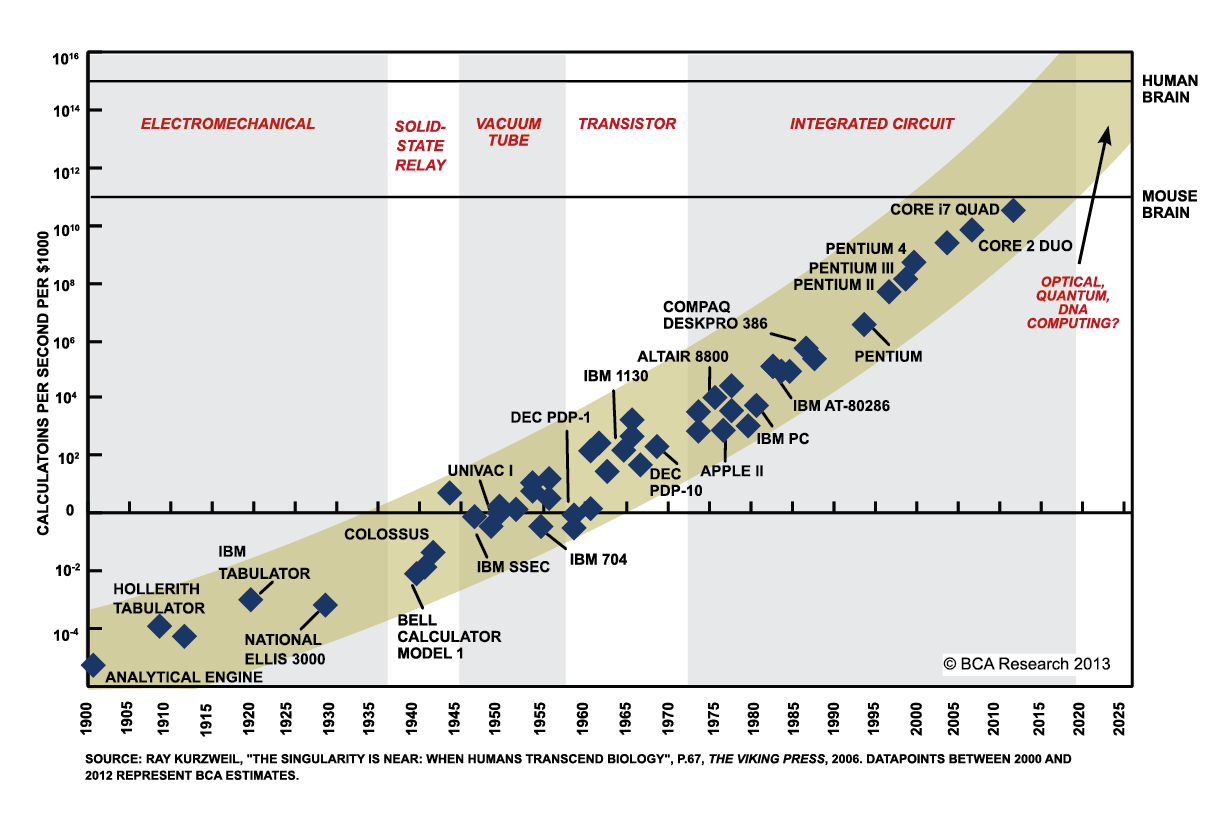
\includegraphics[height=0.47\textwidth, trim=0cm 1.2cm 0 1.2cm,clip=true]{./figs/MooresLaw.png}
\caption{Moore's Law over the years [BCA Blog] \cite{MooreLaw}]}
\label{fig:Moore}
\end{figure}
\end{frame}

%==========================================================================

\subsection[experimental]{Turbulent combustion - experimental}
\begin{frame}%[allowframebreaks]
\frametitle{Turbulent combustion - experimental}
\small{Turbulent combustion: real fluid flows almost always involve turbulence. Large eddy simulation (LES) - technique to achieve higher accuracy than Reynolds' averaged Navier Stokes (RANS) at lower computational cost (time, resources) than direct numerical simulation (DNS).}
\begin{minipage}[0.5\textheight]{\textwidth}
\begin{columns}[T]
\begin{column}{0.65\textwidth}
\vspace{20pt}
\small{Lifted turbulent Ethylene ($C_2H_4$) jet flame issuing into a concentric co-flow of air. Zone between flame-base and nozzle may have partial premixing. Fuel and air temperature, pressure near standard [K{\"o}hler 2006] \cite{Kohler}}
\begin{itemize}%[<+->]
\tiny
\setlength\itemsep{-0.7mm}
\item Dimensions: Nozzle diameter = 2.0 mm; Co-flow air annulus diameter = 140 mm\\
\item Exit Reynolds number: 10000
\item Air mass flow: 320 g/min 
\item Mean fuel jet velocity: 44 m/s 
\end{itemize}
\end{column}

\begin{column}{0.3\textwidth}
\vspace{0pt}
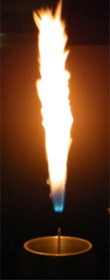
\includegraphics[height=1.4\textwidth]{./figs/dlrflame.png}
\newline
\tiny
[K{\"o}hler 2006] \cite{AdelaideISF}
\end{column}
\end{columns}
\end{minipage}
\end{frame}

%==========================================================================

\subsection[simulation]{Turbulent combustion - simulation}
\begin{frame}%[allowframebreaks]
\frametitle{Turbulent combustion - simulation example}
\scriptsize
{Considering that DNS resolves all the scales, LES models sub-filter scales (SFS) while resolving the larger scales, and that RANS models all the scales, then we can expect the most accurate to be DNS, then LES, then RANS. Computational results that Yang, Pope and Chen  obtained are:}
\vspace{-25pt}
\begin{figure}
\label{fig:DNSLES}
\centering
\subfloat[\tiny{temperature in x-y plane: DNS (l), LES/PDF (r)} \label{fig:contourDNS}]{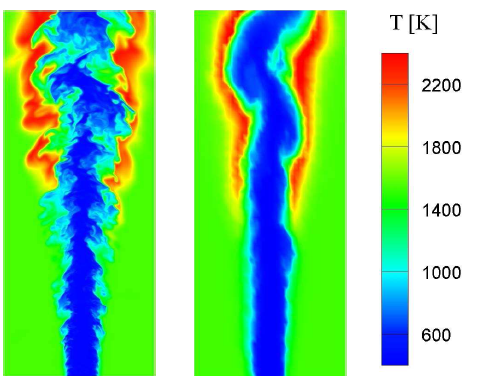
\includegraphics[width=0.7\textheight]{./figs/Temperatures.png}}
\subfloat[\tiny{Mean temperature :DNS and LES} \label{fig:meanTemp}]
{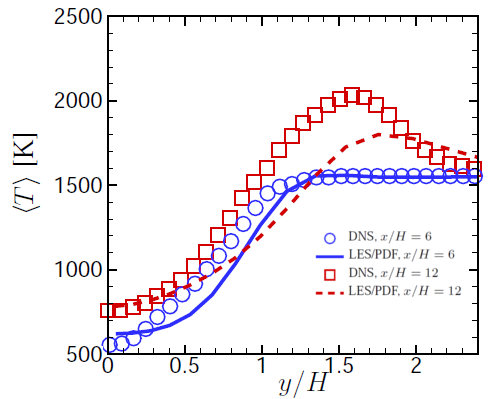
\includegraphics[width=0.65\textheight]{./figs/Temp_DNS_LES2.png}}
\tiny{\caption{\tiny{DNS and LES results for a turbulent Ethylene jet flame in hot co-flow, [Yang et al, 2013 \cite{Pope}]}}}
\end{figure}
\end{frame}

\begin{frame}%[allowframebreaks]
\frametitle{Turbulent combustion - simulation example cont'd}
\scriptsize
Their numerical setup:
\begin{itemize}
\item DNS 
\begin{itemize}
\tiny
\item Grid points $ = 1.3 \times 10^9$.  
\item Computational cost $ = \approx 14 \times 10^6$ CPU hours.
\item Computational domain $ = 3D $ cuboid  $L_x \times L_y \times L_z = 15H \times 20H \times 3H$ in the streamwise x-, transverse y-, and spanwise z-directions, where H = 2 mm is the jet width. Boundary conditions (BCs) are inflow/outflow in x and y, while periodic in z.
\end{itemize}
\item LES
\begin{itemize}
\tiny
\item Grid points $ \approx 8.3 \times 10^3$.  
\item Computational cost $ = $ not specified - expected to be several orders of magnitude \textit{lower}.
\item Computational domain $ = 3D $ cuboid $  L_x \times L_y \times L_z = 15H \times 30H \times 3H$. (larger y to move the transverse boundary away from the central turbulent jet, which can avoid the artifact of the Dirichlet boundary condition on entrainment near the jet.)
\end{itemize}
\end{itemize}
The results they obtained for mean temperature reveal good agreement between LES and DNS at x/H = 6, with lower-than-predicted values at x/H = 12. They anticipate mean temperature prediction to improve with finer mesh resolution in the LES grid.

\end{frame}
%=========================================================================

\section[Methodology]{Methodology}
\begin{frame}%[allowframebreaks]
\frametitle{Scope and methodology within framework}
\scriptsize

\begin{itemize}
\item Reducing numerical error: using high order CENO and adjoint based error estimation : {$\mathcal{O}(h^p)$} $\rightarrow$ h and p adaptation

\item Combustion modeling:
  \begin{itemize}
   \tiny
   \item PCM-FPI: allowing detailed chemical kinetics via tabulation of precomputed laminar premixed flames [H. Perez 2011]
   \end{itemize}  


\item Favre averaged Navier Stokes governing equations

\item Large Eddy Simulation:
  \begin{itemize}
  \tiny
   \item Explicit Filtering [Deconinck 2008]
   \item Sub-filter scale (SFS) modeling [H-Perez 2011]
  \end{itemize}

\item High-order finite volume methods: CENO technique - benefits of higher accuracy on a coarse mesh [Groth and Ivan 2013][Ivan 2010][Rashad 2009]


\item AMR
   \begin{itemize}
   \tiny
   \item Block-based AMR: speed and parallelization [Groth et al 1999]
   \item Anisotropic vs Isotropic: how cell count (computational cost) can be reduced [Zhang 2011][Williamschen 2013][Freret 2015]
   \item Now the non-uniform vs the uniform block modification [Freret 2015]
   \end{itemize}
   
\item Solver: [Northrup 2013] implemented an implicit time marching GMRES method that improves the capability of the CFFC code   
   
\item Creating a framework for the adjoint based error estimation method
\end{itemize}
\end{frame}

%==========================================================================


\section[Error]{Overview of error}
\begin{frame}%[allowframebreaks]
\frametitle{Overview of error}
\vspace{-5pt}
\begin{minipage}[t][0.7\textheight]{1\textwidth}
\scriptsize
\vspace{-20pt}
\begin{block}{Likely sources of error}
\vspace{-10pt}
\begin{figure}[h!]
%\centering
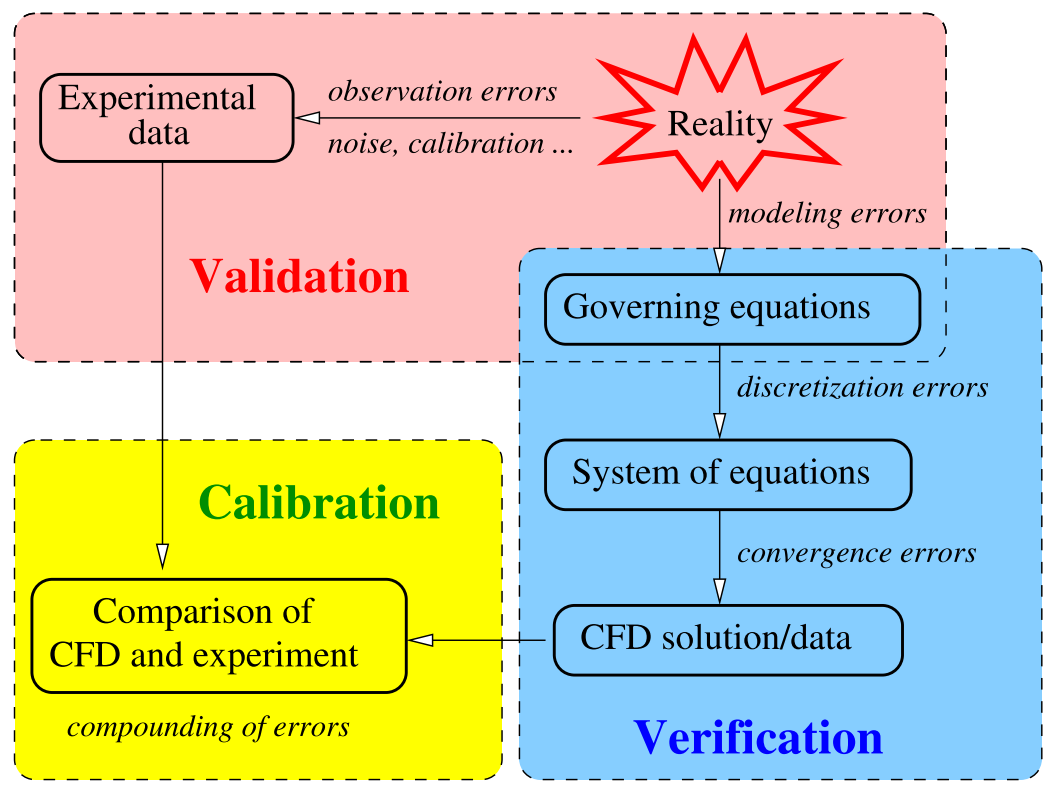
\includegraphics[height=0.47\textwidth]{./figs/Error.png}
\vspace{-5pt}
\caption{Some sources of error [Fidkowski 2012]}
\label{fig:Fidk}
\end{figure}
\vspace{-20pt}
\end{block}
\end{minipage}
\end{frame}


\begin{frame}%[allowframebreaks]
\frametitle{Types of error}
\scriptsize
We can broadly classify the two key sources of error in CFD as follows:

\begin{enumerate}
\item Numerical error:
	\begin{enumerate}[a]
	\scriptsize
	\item Solution error - that between the exact solution value and the CFD obtained value
	\item Truncation error - exists between the actual governing equations and the discretized PDEs for the numerical scheme
	\item Convergence error - arising due to nature of the iterative technique used
	\end{enumerate}
\item Modeling error:
	\begin{enumerate}[a]
	\scriptsize
	\item Pertaining to LES:
		\begin{itemize}
		\tiny
		\item Sub-filter scale turbulence model: inappropriate model selected
		\item Combustion and chemistry model
		\item Filtering:\newline
			  aliasing errors - decomposed nonlinear terms in FANS = feedback of frequencies beyond filter bandwidth, = 'fake' stresses \newline
			 commutation errors - exist between filtering and differential operations 
		\end{itemize}
	\item Errors in geometry definition 
	\item Errors in types of mesh cells - selection of the mesh refinement, types of cells, configuration to bulk flow direction
	\end{enumerate}
\end{enumerate}

\end{frame}


%==========================================================================

\section[AMR]{Adaptive mesh refinement}

\subsection{Basis}
\begin{frame}%[allowframebreaks]
\frametitle{Adaptive mesh refinement (AMR)}
\tiny
\begin{minipage}[t][1\textheight]{1\textwidth}
\vspace{-15pt}
\begin{exampleblock}{Key characteristics}
AMR: [Berger et al 1984, 1986, 1989] [Aftomis et al 1998, 2000, 2004]
\begin{itemize}
\tiny
\item localized refinement, large variation of scales, easily automatable
\end{itemize}
\vspace{-20pt}
\begin{figure}
\label{fig:cubeAMRbased}
\centering
\subfloat[\tiny{Cell refinement strategies on a reference uniform mesh[Zhang 2011]} \label{fig:blockdiv}]
{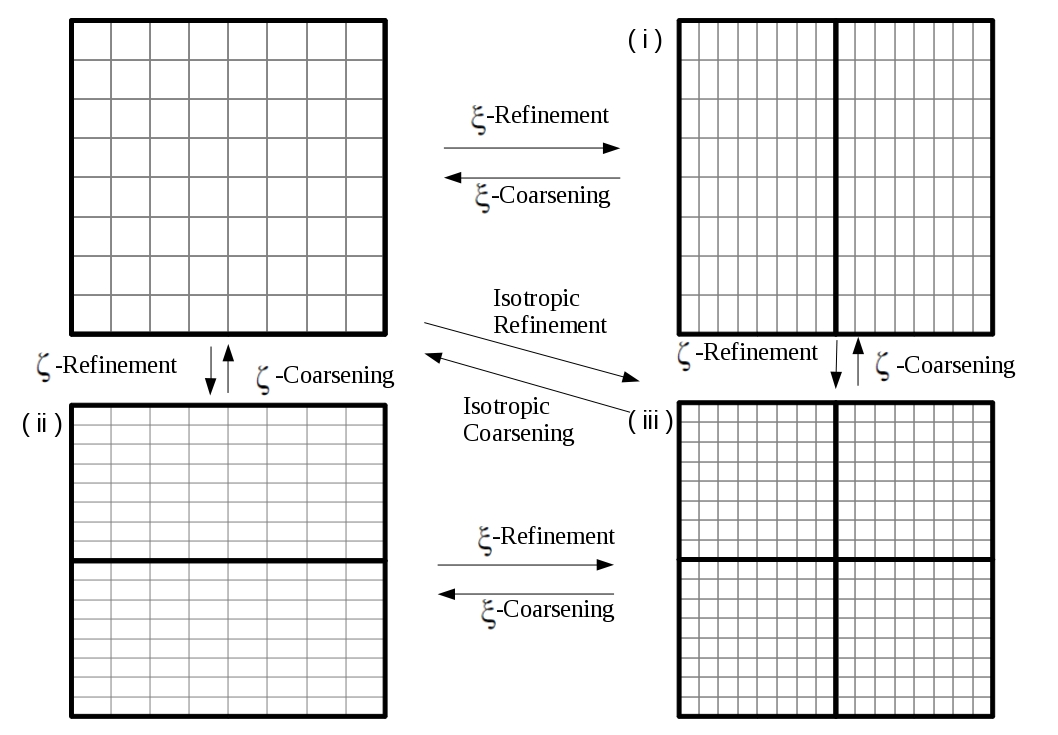
\includegraphics[width=1\textheight, trim=0cm 0cm 0 0cm,clip=true]{./figs/BlockDivision.jpg}}
\end{figure}
\vspace{-15pt}
\begin{itemize}
\tiny
\item Benefits of AMR: overall large computational cell count savings
\end{itemize}

\end{exampleblock}
\end{minipage}

\end{frame}

%---------------------------------------------------------------------------------------

\subsection{Block based AMR}
\begin{frame}%[allowframebreaks]
\frametitle{Block based AMR}
\tiny
\begin{minipage}[t][1\textheight]{1\textwidth}
\vspace{-15pt}
\begin{exampleblock}{Key characteristics}
Block-based AMR: [Groth and co-workers 1999, 2005, 2006, 2010, 2011, 2012] \newline
Entire block gets refined, along with all its cells. This approach is much cheaper than individual cell refinement, since the latter would require updated lists and cross-checking.
\vspace{-20pt}
\begin{figure}
\label{fig:cubeAMRbased}
\centering
\subfloat[\tiny{With Anisotropic AMR. 5522 (8x8x8) blocks [Freret 2015]} \label{fig:cubeIso}]
{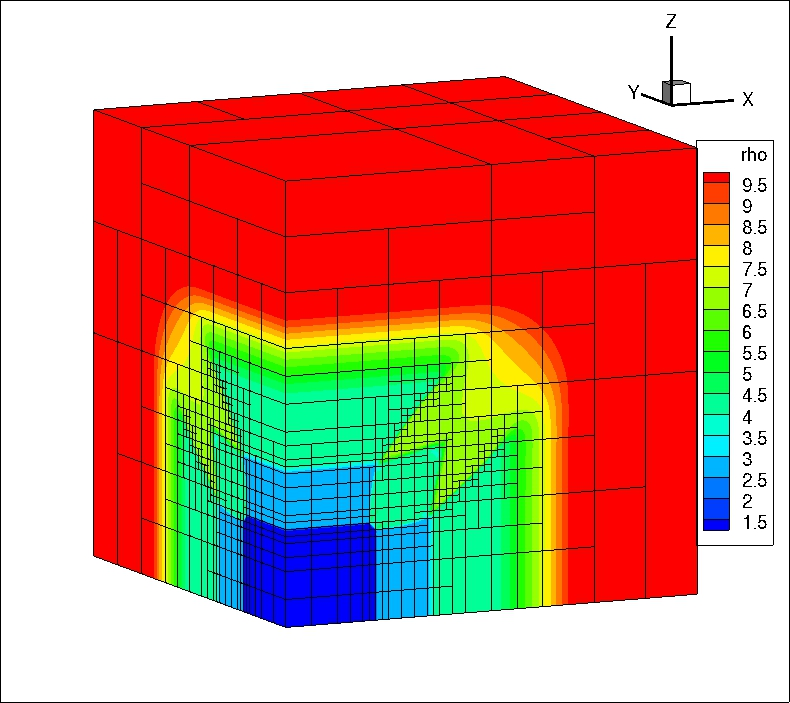
\includegraphics[width=0.6\textheight, trim=0cm 0cm 0cm 0cm,clip=true]{./figs/shockCubeAniso3.jpg}}
\subfloat[\tiny{With isotropic AMR. 7036 (8x8x8) blocks [Freret 2015]} \label{fig:cubeAniso}]
{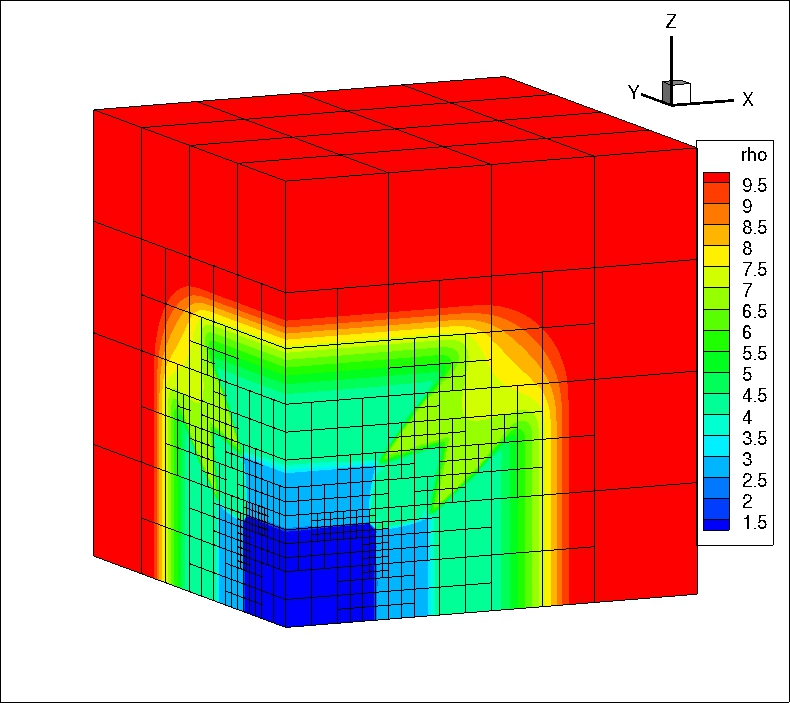
\includegraphics[width=0.6\textheight, trim=0cm 0cm 0 0cm,clip=true]{./figs/shockCubeIso3.jpg}}
\end{figure}
\vspace{-15pt}
\begin{itemize}
\tiny
\item Isotropic vs anisotropic: up to 85\% savings in cell count in 3D [Williamschen 2013]
\end{itemize}
\end{exampleblock}
\end{minipage}

\end{frame}

%---------------------------------------------------------------------------------------



\subsection{Usage}
\begin{frame}%[allowframebreaks]
\frametitle{Implementation}
\tiny
\begin{minipage}[t][1\textheight]{1\textwidth}
\vspace{-15pt}
\begin{exampleblock}{Key characteristics}
[Groth and co-workers 1999, 2005, 2006, 2010, 2011, 2012, 2013]:
\begin{itemize}
\tiny
\item How the block-based technique works; ghost cells for intercommunication 
\item Parallelizable, low memory and storage requirements
\item New non-uniform approach [Freret 2015]
\end{itemize}

\vspace{-15pt}
\begin{figure}
\label{fig:Blockbased}
\centering
\subfloat[\tiny{Ghost cells on 8 blocks [Rashad 2009]} \label{fig:2dcomm}]
{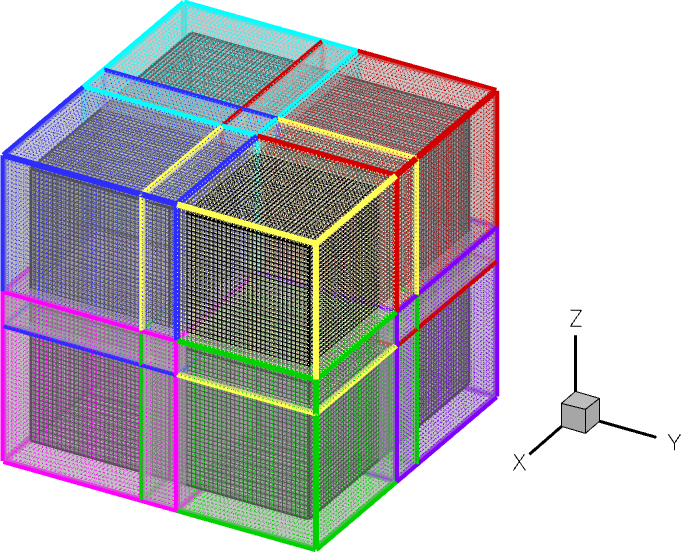
\includegraphics[width=0.4\textheight, trim=0cm 0cm 0cm 0cm,clip=true]{./figs/ghostblock.png}}
\subfloat[\tiny{Parallelization [Northrup 2013]} \label{fig:parall}]
{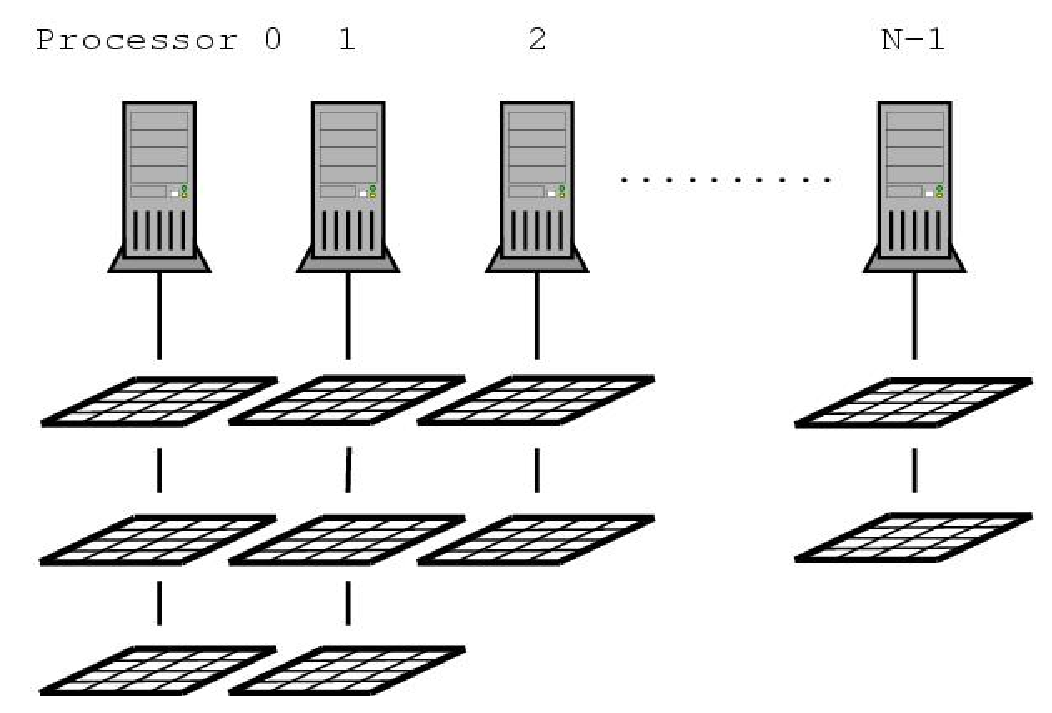
\includegraphics[width=0.4\textheight, trim=0cm 0cm 0 0cm,clip=true]{./figs/parallel-domain-decomp.eps}}
\subfloat[\tiny{Non-uniform approach [Freret 2015]} \label{fig:nonUni}]
{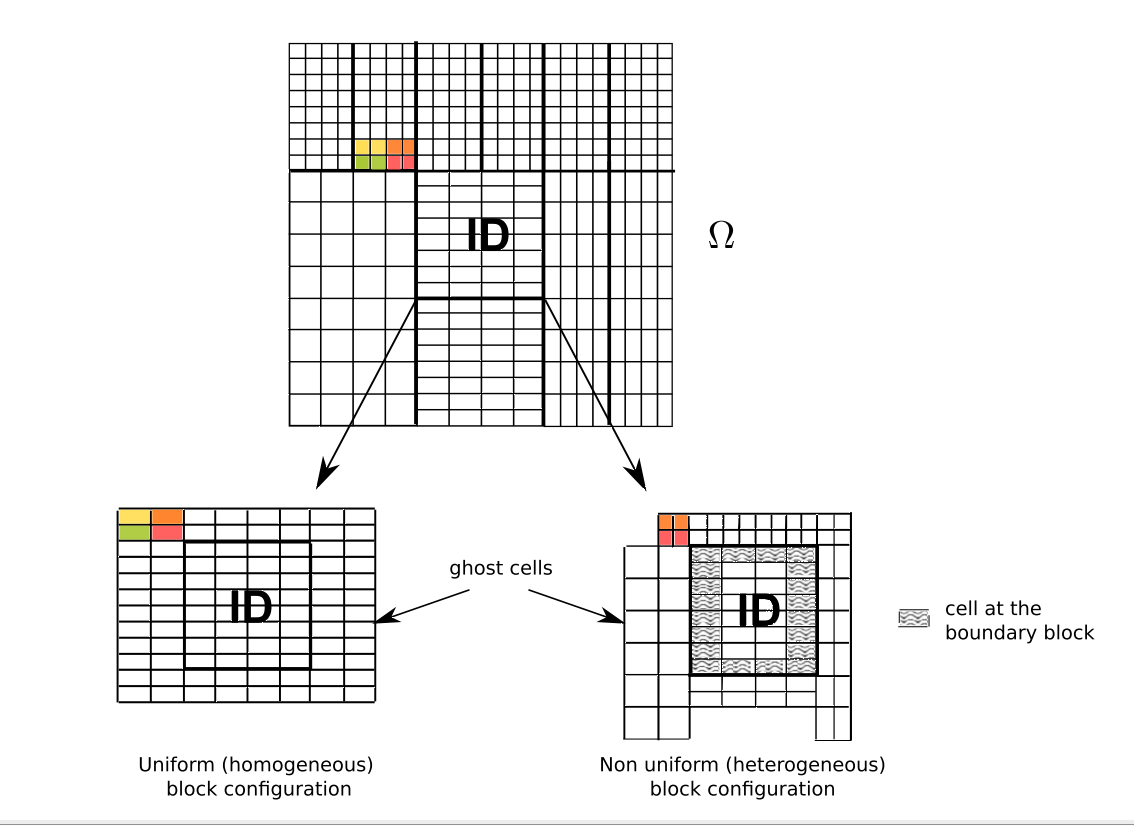
\includegraphics[width=0.55\textheight, trim=2cm 0cm 1cm 0cm,clip=true]{./figs/Non-UniformBlock.png}}
\end{figure}
\vspace{-15pt}
\end{exampleblock}
\end{minipage}

\end{frame}





%==========================================================================

\section[FVM]{High order FVM, CENO and LES}
\subsection{High order FVM}
\begin{frame}%[allowframebreaks]
\frametitle{High order finite volume method}
\begin{minipage}[t][1\textheight]{1\textwidth}
\vspace{-20pt}
\begin{exampleblock}{Error reduction via p}
\tiny

An explanation on h.o FVM.  $ p > 2 $.

\begin{block}{Integral Form of the Governing Equations}
     \[
      \frac{\mathrm{d}\overline{\mathbf{U}}}{\mathrm{d}t} = 
      - \frac{1}{V} \oiint_A \left( \vec{\mathcal{F}}^{\rm I} - 
      \vec{\mathcal{F}}^{\rm V} \right) \cdot \hat{n} \mathrm{d}\mathcal{A} + 
      \overline{\mathbf{S}}
     \] 
    Using a two-dimensional Gauss quadrature integration rule:
    \[  \frac{\mathrm{d}\overline{\mathbf{U}}_{ijk}}{\mathrm{d}t} = 
       \frac{1}{{V}_{ijk}} \sum_{l=1}^{N_f}     
      \sum_{m=1}^{N_G} \left( \omega \left(\vec{\mathcal{F}^{\mathrm{I}}} - 
      \vec{\mathcal{F}^{\mathrm{V}}} \right)\cdot \hat{n} {A} \right)_{ijk,l,m} 
      + \overline{\mathbf{S}}_{ijk} 
      = \overline{\mathbf{R}}_{ijk}  \left( \overline{\mathbf{U}} \right) \]
    The higher the order p of the scheme, the more the quadrature points ($ N_G $) which have their own corresponding weights $ \omega $.
\end{block}


\begin{itemize}
\tiny
\item Gauss-Legendre quadrature rules are defined on reference cartesian cubic elements, and mapped onto 3D hexahedral elements via mapping functions
\item High-order schemes reduces numerical error by increasing the accuracy of approximation between the actual governing equations (PDE form) and the discretized value.
\item Other groups researching this: Ihme (Stanford) and Poinsot (CERFACS)
\end{itemize}
\end{exampleblock}
\end{minipage}


\end{frame}

%---------------------------------------------------------------------------------

\subsection{CENO}
\begin{frame}
\scriptsize
\frametitle{Central essentially non-oscillatory (CENO) scheme implementation} 

\begin{minipage}[t][1\textheight]{1\textwidth}
\vspace{-20pt}
\begin{exampleblock}{Error reduction via p}
\tiny
[Ivan and Groth 2011, 2012]
\begin{itemize}
\item CENO eliminates oscillations that are typical of discontinuities
\item Reconstruction: FVM technique is cell centered. We may at times need state values on faces (flux evaluations) or at quadrature points (high-order)
\item CENO uses fixed stencil for reconstruction
\item smoothness indicators are used to select if a high order (p) reconstruction is to be carried out, or just a piecewise linear reconstruction
\end{itemize}
\vspace{-20pt}
\tiny
\begin{figure}
\label{fig:h_order_error}
\centering
\subfloat[\tiny{Example of quadrature points on the cell faces} \label{fig:errorHO}]
{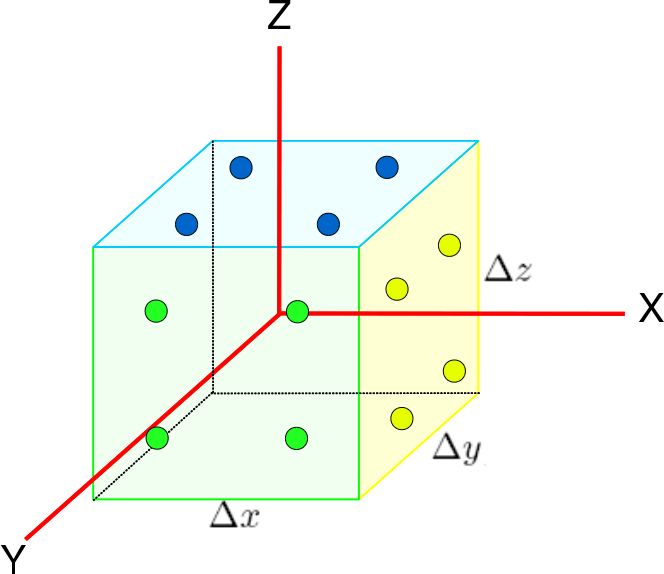
\includegraphics[width=0.53\textheight, trim=0cm 0cm 0cm 0cm,clip=true]{./figs/fig_quadpts.png}}
\subfloat[\tiny{L1 error norm in the solution for an unsteady advection equation having a quantity distribution gaussian profile. N = total mesh count} \label{fig:errorHO}]
{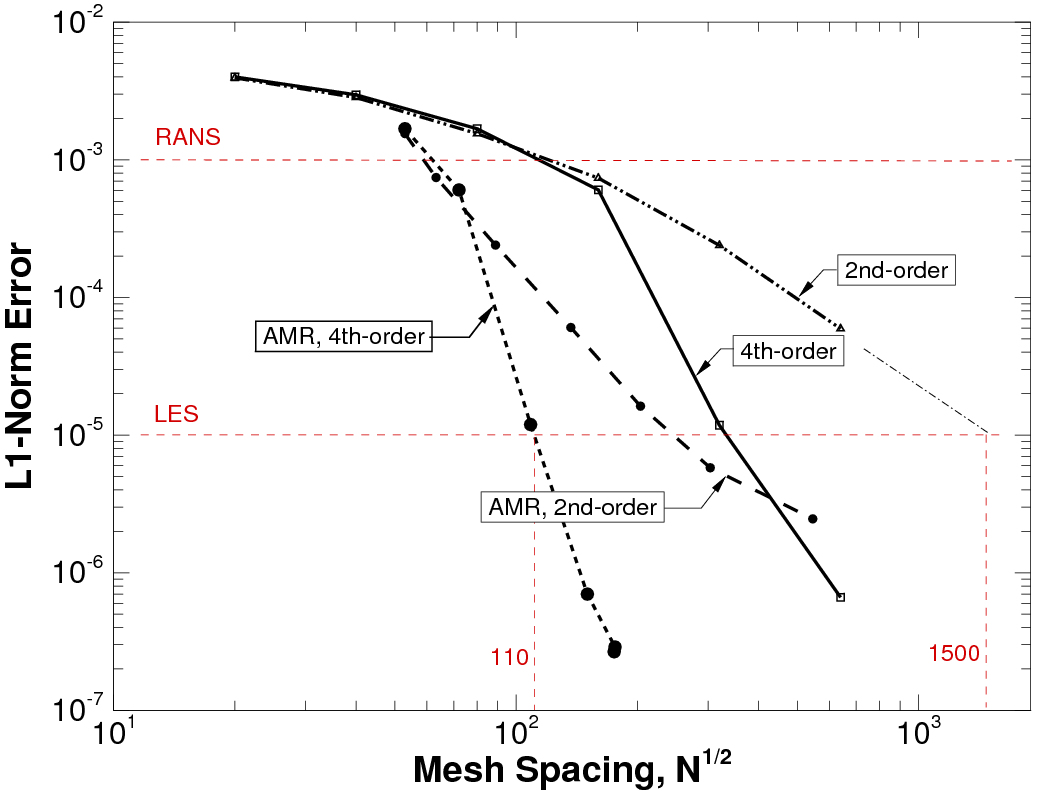
\includegraphics[width=0.6\textheight, trim=0cm 0cm 0cm 0cm,clip=true]{./figs/error_ho_amr3.jpg}}
\end{figure}
\end{exampleblock}
\end{minipage}

\end{frame}

%------------------------------------------------------------------------------


\subsection{LES}
\begin{frame}
\frametitle{Large Eddy Simulation (LES)}
\scriptsize
[Piomelli 1999][Ghosal and Moin 1999]
\begin{itemize}
\item The accuracy of LES lies between the very accurate DNS and RANS.
\item DNS is mostly impractical and very expensive
\item RANS has fully modelled turbulence. Only the largest scales are resolved
\item LES utilizes a spatial filtering of a given width, $\bar{\Delta} $. Any scales below this will be modelled $\rightarrow$ sub-filter scales (SFS) [Smagorinsky 1963][Germano 1991][Piomelli 1991][Ghosal and Moin 1999][Lilly 1992]
\item while scales larger than $\bar{\Delta}$ will be fully resolved.

\item Hence in LES an appropriate balance is sought for accuracy, since too much reliance on modeling can be a source of error. Can be broadly categorized into two:

\begin{itemize}
\tiny
\item Implicit filtering [Aspden et al 2008]
\begin{itemize}
\tiny
\item The filter width is not explicitly defined
\item Inherently related to grid resolution
\item Main disadvantage - difficult to compare results of adapted/refined meshes
\item Difficult to control aliasing and commutation errors
\end{itemize}


\item Explicit filtering. [Vasilyev et al, 1998] [Deconinck, 2008]
\begin{itemize}
\tiny
\item Define $\bar{\Delta} $ to be fixed for the entire mesh: top-hat, Gaussian, etc.
\item Results easily comparable since $\bar{\Delta} $ does not change for different meshes
\item Order of truncation errors (discretized scheme) can be controlled to be the same order of the commutation errors
\item Allows control of aliasing errors
\end{itemize}

\end{itemize}

\end{itemize}
\end{frame}


%===== ADJOINT =====================================================================
\section[Error estimates]{Error estimation}

\subsection{Foundation}
\begin{frame}
\frametitle{Foundation for error estimation}
\scriptsize
Basis for selective mesh refinement - we would like to refine the mesh where the cells have a very critical effect on the solution, while coarsening the less critical areas to save on computational cost.\newline 
Basically, there are two types of error estimation procedures available:
\begin{itemize}
\item a priori error estimators:  these predict the long-term behavior of the errors in the discretization. They are not actually designed to approximate the error estimate for a given mesh. 
\item a posteriori error estimators: these use the simulation results to derive estimates of solution errors. Furthermore, these results are used to guide adaptive schemes:
\begin{itemize}
\scriptsize
\item where either the mesh is locally refined (h-version) 
\item where the polynomial degree is raised (p-method)
\end{itemize}
\end{itemize}
Two main a posteriori approaches are the:
\begin{itemize}
\item gradient-based : [Bibb et al, 2006] [Giles and Pierce, 2000]
\item adjoint-based : [Giles and Pierce, 2000][Venditti and Darmofal - 2000,2002][Fidkowski and Darmofal, 2011] 
\end{itemize}
\end{frame}


\subsection[Gradient]{A background on gradient/physics-based refinement}
\begin{frame}%[allowframebreaks]
\scriptsize
\frametitle{A background on gradient/physics-based refinement}
In these simulations, the mesh or discretization order is changed based on the rates of change of (physical) solution variables.\newline
Where the change occurs most rapidly over a few mesh cells, then over this location the mesh resolution can be increased (higher mesh refinement), or the scheme order can be increased, effectively using a higher order discretization over these cells.

\begin{itemize}
\item The reasoning behind this is to have enough cells to capture the changes as \textit{smoothly} as possible.
\item Once refinement is completed, the solution is re-run and the gradients re-evaluated. Changes made as necessary. Error can be compared to a higher discretization (h or p) solution.
\item This is the present utility in the anisotropic and isotropic AMR functionality of the CFFC code used by the CFD and Propulsion group.
\item main disadvantages of the gradient based approach [Giles and Pierce, 2000]:
\begin{itemize}
\tiny
\item for each separate state variable, a separate simulation must be run to evaluate the desired mesh resolution - increases computational time
\item gradient-based approach can only deal with continuous functionals as opposed to discrete optimization functionals
\item inability to deal with functions that have multiple minima. In this latter case, the gradient-based technique will generally converge to the nearest local minima, whose value may not represent overall system minimum.
\end{itemize}
\end{itemize}
\end{frame}

%-----------------------------------------------------------------
\subsection[example]{CFFC example}
\begin{frame}
\frametitle{Example of gradient-based mesh refinement}
\scriptsize
\begin{minipage}[t][1\textheight]{1\textwidth}
\vspace{-10pt}
\begin{exampleblock}{Physics as criteria for mesh coarsening/refinement - sphere with a bow shock example}
\vspace{-20pt}
\begin{figure}
\label{fig:Gradientbased}
\centering
\subfloat[\tiny{With isotropic AMR} \label{fig:sphereIso}]
{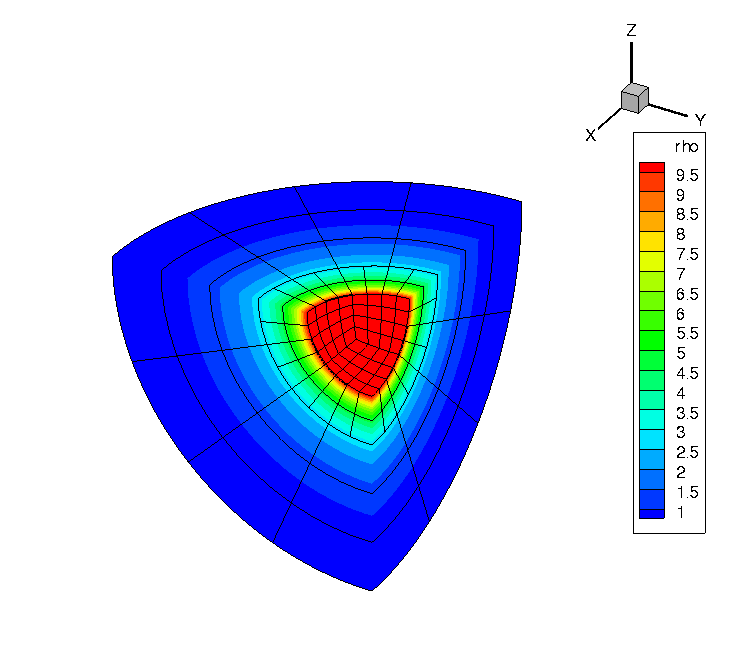
\includegraphics[width=0.45\textheight, trim=0cm 0cm 0cm 0cm,clip=true]{./figs/outflowIso.png}}
\subfloat[\tiny{With anisotropic AMR} \label{fig:sphereAniso}]
{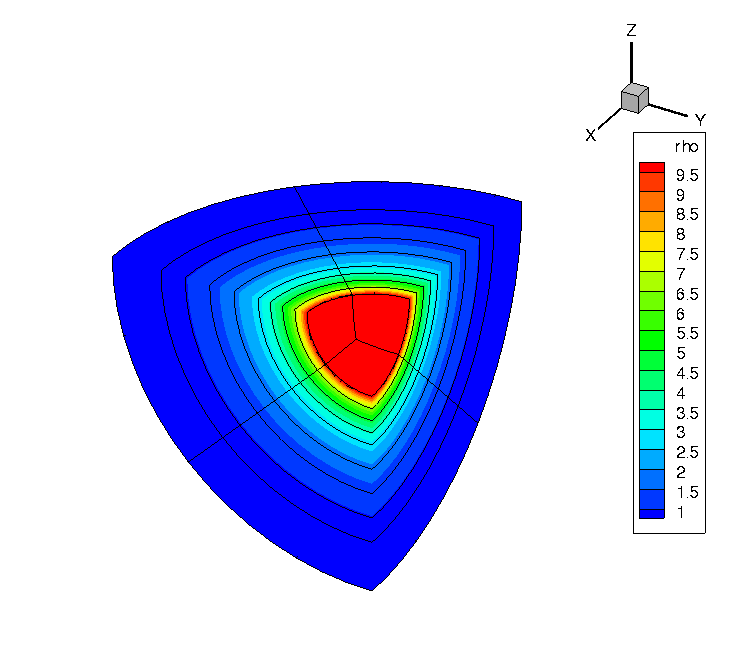
\includegraphics[width=0.45\textheight, trim=0cm 0cm 0 0cm,clip=true]{./figs/outflowAniso.png}}
\subfloat[\tiny{Error in the density norm} \label{fig:rhoError}]
{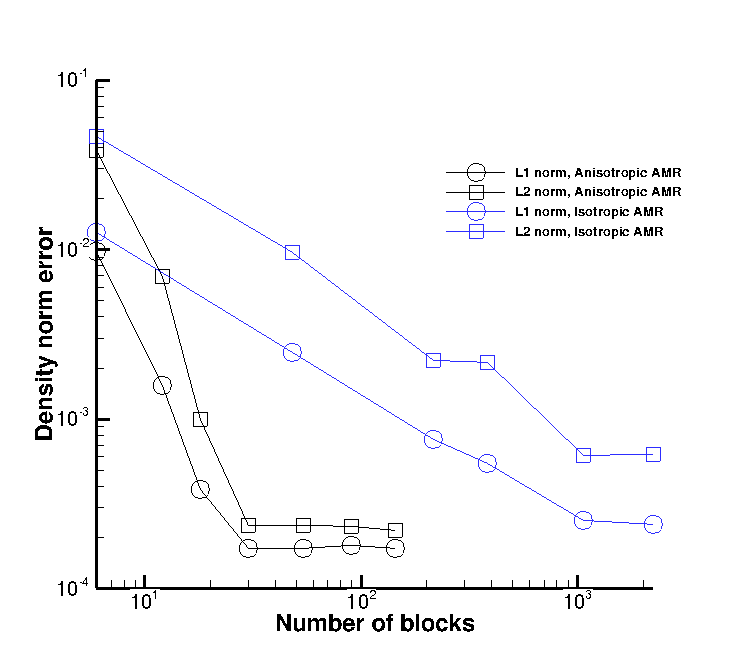
\includegraphics[width=0.45\textheight, trim=0cm 0cm 0 0cm,clip=true]{./figs/outflowError.png}}
\end{figure}

[Freret, 2015] and [Williamschen, 2013]
\begin{itemize}
\item The graph reveals the asymptotic behavior of the convergence, yet for increased number of cells, there should be continual reduction in the density error norm
\end{itemize}
\end{exampleblock}
\end{minipage}

\end{frame}



\subsection[Adjoint]{About the adjoint}
\begin{frame}%[allowframebreaks]
\scriptsize
\frametitle{About the adjoint}
To make error estimation more relevant to engineering applications: assess the error made in predicting an integral quantity which represents an engineering output. This output is the functional. For example,the output can be the average pressure on a wall. 
\newline The adjoint technique is a sensitivity analysis, that measures the rates of change of a design functional to a given change in the input. (It is a function of the residual, but the residual is in turn a function of both the input and the state). \newline
The adjoint has two main formulations [Giles and Pierce: 1997,2001][Jameson, 2001][Venditti and Darmofal, 2000, 2002] [Becker and Rannacher: 2001,2003]:
\begin{itemize}
\item continuous:
\begin{itemize} 
\tiny
\item An objective function is formed to enforce the flow conditions (i.e. primal nonlinear PDEs). 
\item Consider linear perturbations to the primal flow variables: the objective function should remain constant w.r.t the perturbations.
\item Hence obtain analytical adjoint equations. Obtain appropriate boundary conditions, and discretized directly. Primary benefit - offers insight into the nature of the adjoint solution.
\end{itemize}
\item discrete 
\begin{itemize}
\tiny
\item begin with the nonlinear discrete residual equations from the primal problem
\item apply linear perturbations to these. 
\item If adjoint consistent (discrete adjoint = continuous adjoint), no need for B.C. specification -automatically incorporated via the primal residual.   
\item thus obtain a linear system of equations - only need linear sensitivities of the functional and the Jacobian matrix associated with the primal residual.
\end{itemize}
\end{itemize}
\end{frame}

\begin{frame}
\frametitle{Discrete adjoint}
\scriptsize
For these initial stages, beginning with the discrete formulation of the adjoint
\begin{minipage}[t][0.6\textheight]{1\textwidth}
\scriptsize
\vspace{-10pt}
\begin{exampleblock}{Discrete Adjoint}
\[\left( \frac{\partial{R}}{\partial{U}} \right)^T ~\Psi~ = -\left( \frac{\partial{J}}{\partial{U}} \right)^T\]
\text{yielding a linear system of equations:}
\vspace{-10pt}
\[Ax = b\]
\vspace{-10pt}
\text{Where:}
\vspace{10pt}
\begin{itemize}
\item \textbf{$J$} = the functional
\item \textbf{$R$} =  the residual
\item \textbf{$\psi$} = the adjoint vector
\end{itemize}
\end{exampleblock}
\end{minipage}

Methods to evaluate the matrix $\frac{\partial{R}}{\partial{U}} $  for the discrete adjoint:
\begin{itemize}
\scriptsize
\item Finite differencing - perturbing the state U to evaluate R 
\item Automated differentiation - tools that evaluate the differential [Bischof et al: 1992, 1996, 2008]
\item Approximate method  - using the inbuilt functions within CFFC code [Northrup, 2013]
\item Complex step [Martins, Alonso and Sturdza: 2003]
\end{itemize}


\end{frame}


%=====================================================================

\subsection[Usage]{Basis of refinement: h and p}
\begin{frame}%[allowframebreaks]
\frametitle{\scriptsize{Usage of the adjoint as a basis of refinement: h and p}}
\scriptsize
Some of the groups using \textbf{adjoint with AMR}
\begin{itemize}
\item Becker and Rannacher [2001] - An Optimal Control Approach to a Posteriori Error Estimation in Finite Element Methods
\item Fidkowski and Darmofal [2011] - Review of Output-Based Error Estimation and Mesh Adaptation in Computational Fluid Dynamics
\item Hartmann [2006] - Error Estimation and Adjoint-based Adaptation in Aerodynamics
\item Nemec and Aftosmis [2007] - Adjoint Error Estimation and Adaptive Refinement for Embedded-Boundary Cartesian Meshes
\item Nemec, Aftosmis, and Wintzer [2008] - Adjoint-Based Adaptive Mesh Refinement for Complex Geometries
\item Hartmann, Held and Leicht [2010] - Adjoint-based error estimation and adaptive mesh refinement for the RANS and k-ω turbulence model equations
\item Woopen, May and Sch{\"u}tz [2013] - Adjoint-Based Error Estimation and Mesh Adaptation for Hybridized Discontinuous Galerkin Methods
\item Li, Allaneau and Jameson [2011] - Continuous Adjoint Approach for Adaptive Mesh Refinement
\item Diskin and Yamaleev [2011] - Grid Adaptation Using Adjoint-Based Error Minimization
\end{itemize}
\end{frame}

%-----------------------------------------------------------------

\subsection[Estimation]{Error estimation indicators}
\begin{frame}
\scriptsize
\frametitle{Error estimation indicators}
[Venditti and Darmofal 2000][Fidkowski and Darmofal 2011]

\begin{itemize}
\item Our goal is to reduce discretization errors based on the mesh resolution.

\begin{itemize}
\tiny
\item Consider 2 levels of mesh resolution: coarse (H) and fine (h). We calculate the state ($U_H$) and functional ($J_H(U_H)$) on the coarse space. Residual, $R_H(U_H) = 0$
\item We would like to evaluate the functional on the fine space, $J_h(U_h)$ (expensive). Thus we use a prolongation operator ($U_h^H = I_h^H U_H$) to inject the fine space state onto the coarse space state.
\item The output error, $\delta J \equiv J_H(U_H) - J_h(U_h) \neq 0$
\item Expect the new residual, $R_h(U_h^H) \neq 0$ 
\item The injected coarse state solves: $ R_h(U_h^\prime) - R_h(U_h^H) = 0 \rightarrow (U_h^\prime) = (U_h^H)$
\item $ \delta J \approx  J_h(U_h^H) - J_h(U_h) = \Psi_h^T \delta R_h = -\Psi_h^T R_h(U_h^H)   $, using the definition of the fine space adjoint, $\Psi_h$
\item Error estimate is the value of $\delta J$, and does not need evaluation of $U_h$, primal solution on the fine space. We can use this error estimate as a flag for refinement, given some threshold value
\end{itemize}

\item Steady vs unsteady adjoints: for unsteady, march forward in time, evaluating $\psi$, then march backwards in time. Now have all the sensitivities. Use this to refine the mesh at those time levels. Check set tolerance and repeat until convergence.
\item Expected benefits of adjoint vs gradient based methods: the adjoint technique is a one time calculation for the sensitivity of a single output to several inputs.
\end{itemize}

\end{frame}

%==========================================================================
\section[Usage]{Usage}

\begin{frame}%[allowframebreaks]
\frametitle{How we can use this: \LARGE{$\mathcal{O}(h^p)$}}

\scriptsize
\begin{itemize}
\vspace{-25pt}
\item h: using error estimates for mesh adaptation. Entire block would be refined.
\begin{minipage}[t][0.7\textheight]{0.95\textwidth}
\vspace{-10pt}
\begin{exampleblock}{Launch abort vehicle example, [Nemec et al, 2008]}
\tiny
Functional as a linear combination of normal and axial forces. $M = 1.1; \alpha=-25\deg$
\vspace{-10pt}

\begin{figure}
\label{fig:LAVone}
\centering
\subfloat[\tiny{Adjoint of density with accompanying error estimate} \label{fig:LAVerror}]
{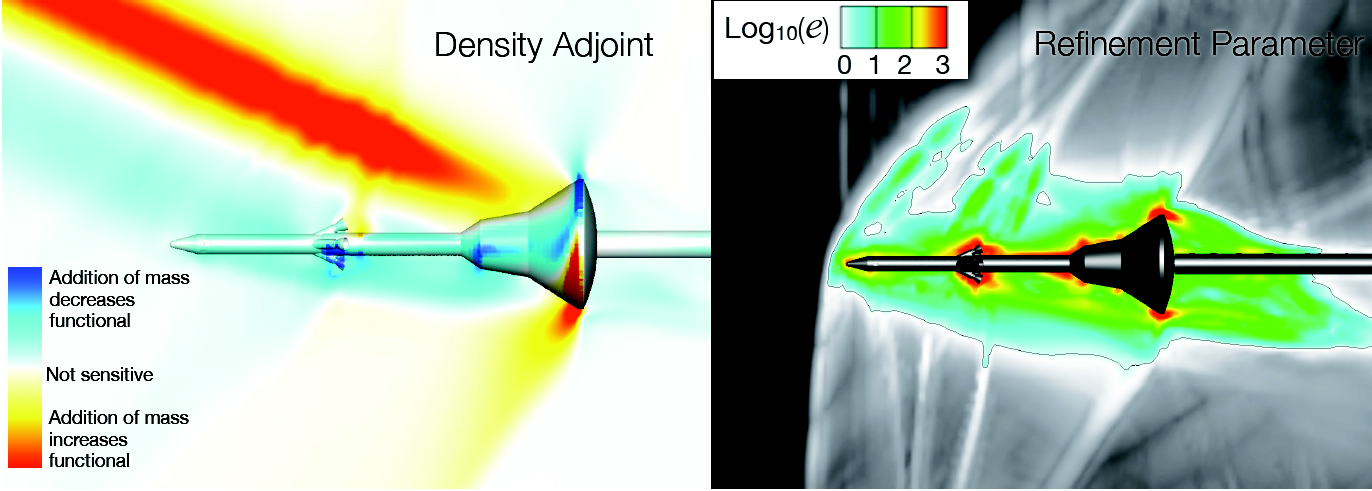
\includegraphics[width=0.5\textheight, trim=0cm 0cm 0cm 0cm,clip=true]{./figs/LAV_adj_err.png}}
\subfloat[\tiny{Final obtained mesh. Initial was $3.7x10^3$ cells; final $2x10^6$ cells } \label{fig:LAVmesh}]
{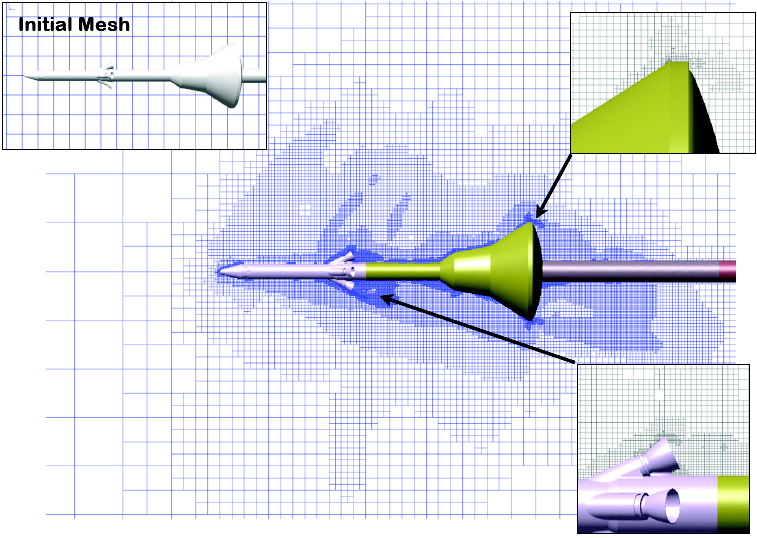
\includegraphics[width=0.7\textheight, trim=0cm 0cm 0cm 0cm,clip=true]{./figs/LAV_mesh.png}}
\end{figure}
\end{exampleblock}
\end{minipage}
\vspace{0pt}
\item p: using the error estimates to run, locally, on the flagged block, a higher discretization of the numerical scheme. Usually, for high order,  $ p > 2 $.


\end{itemize}
\end{frame}


%==========================================================================
\section[Progress]{Progress to date}

\subsection{Poisson}
\begin{frame}[shrink=20]%[allowframebreaks]
\frametitle{Poisson problem}
\scriptsize
\begin{minipage}[t][1\textheight]{1\textwidth}
\vspace{-20pt}
\begin{exampleblock}{Creating and solving linear systems in parallel implementation - trilinos and MPI}
\vspace{-20pt}
\begin{figure}
\label{fig:Poisson}
\centering
\subfloat[\tiny{2D case on $N^2 = 200^2$} \label{fig:Poiss2D}]{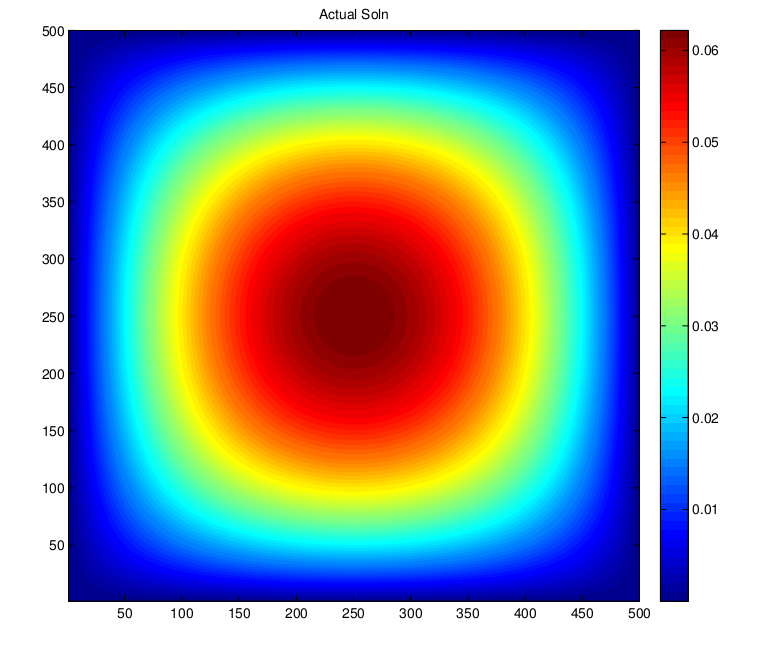
\includegraphics[width=0.7\textheight]{./figs/Poisson2D.png}}
\subfloat[\tiny{3D case on $N^3 = 100^3$} \label{fig:Poiss3D}]{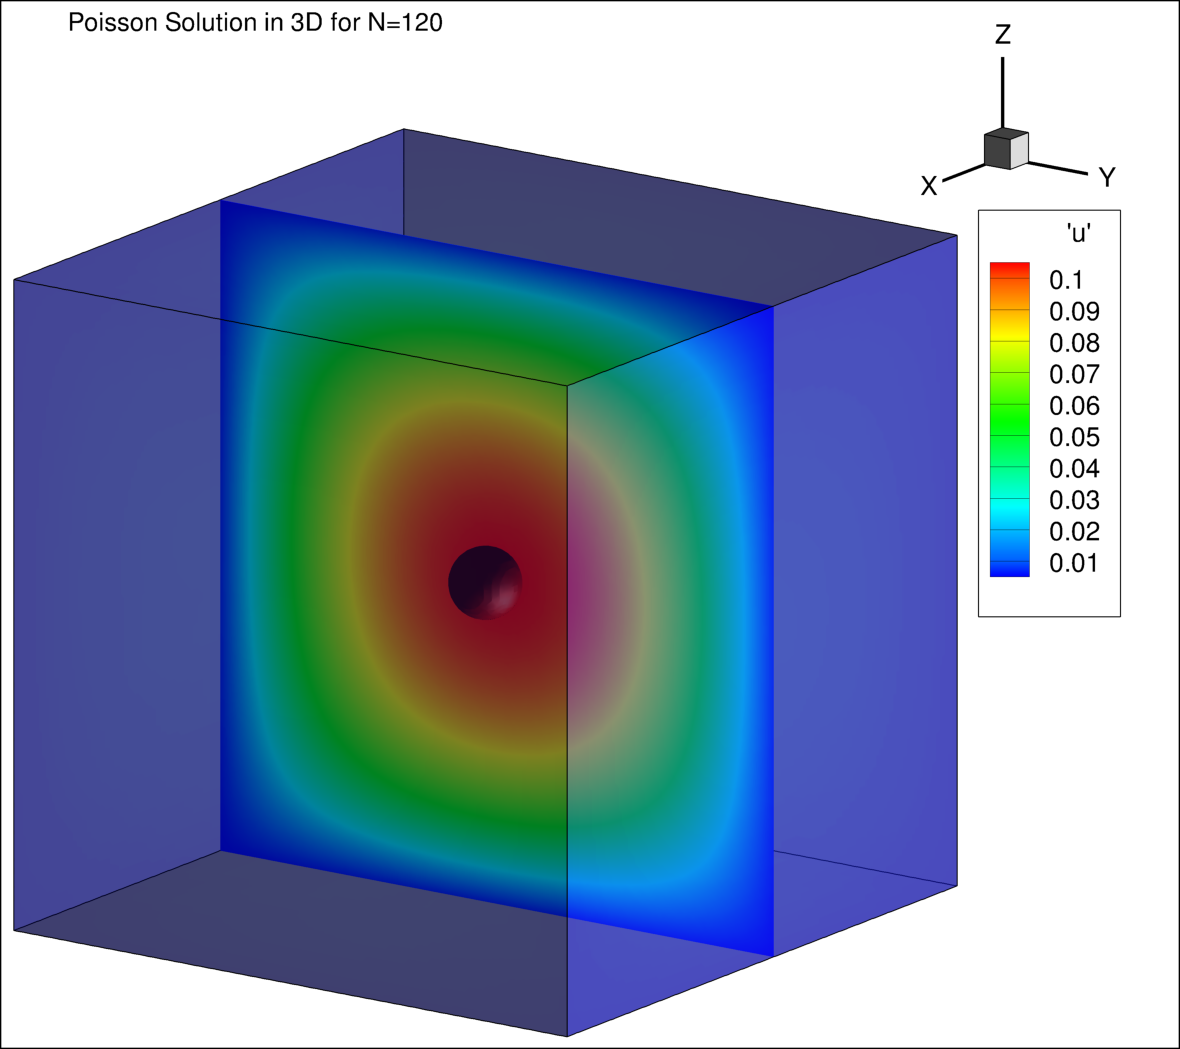
\includegraphics[width=0.7\textheight, trim=0cm 0cm 0 2cm,clip=true]{./figs/3D_Poisson.png}}
\tiny{\caption{\tiny{Solution contours for Poisson problem}}}
\end{figure}
\tiny
\vspace{-15pt}
\[ \text{In 2D:} D=[0,1]^2 , f(x,y)=2(x(1-x)+y(1-y)) \text{ is the source term and }  u(x,y) \text{ is the solution to be computed.} \]
\[\text{Using a } 2^{nd} \text{ order centered finite difference scheme= } -\frac{u_{i+1,j}+u_{i-1,j}+u_{i,j+1}+u_{i,j-1}-4*u_{ij}}{h^2}=f_{ij} \]
\vspace{-5pt}
\[\text{In 3D:} D=[0,1]^3,  f(x,y,z)=3(x(1-x)+y(1-y)+z(1-z)) \text{ is the source term and } u(x,y,z)  \text{ is the solution to be computed.}\]
\[ \text{Using a } 2^{nd} \text{ order centered finite difference scheme:} \]
\[{-\frac{u_{i+1,j,k-1}+u_{i-1,j,k-1}+u_{i,j+1,k-1}+u_{i,j-1,k-1} + u_{i+1,j,k+1}+u_{i-1,j,k+1}+u_{i,j+1,k+1}+u_{i,j-1,k+1}-6 u_{ijk}} {h^2} = f_{ijk}} \]

\end{exampleblock}

\end{minipage}
\end{frame}

%---------------------------------------------------------------------------------------------

%------------------------------------------------------------------------

\subsection{LES flame}
\begin{frame}
\frametitle{Running already existing LES case on SciNET}
\scriptsize
CFFC code familiarization : LES test case - on parallel clusters - SciNET. Job scheduling and post-processing results (tecplot)
\begin{minipage}[t][1\textheight]{1\textwidth}
\vspace{-10pt}
\begin{exampleblock}{Turbulent premixed $CH_4$ flame, $\phi=0.7$. }
\vspace{-20pt}
\begin{figure}
\label{fig:LES}
\centering
\subfloat[\tiny{Flame temp} \label{fig:flametemp}]{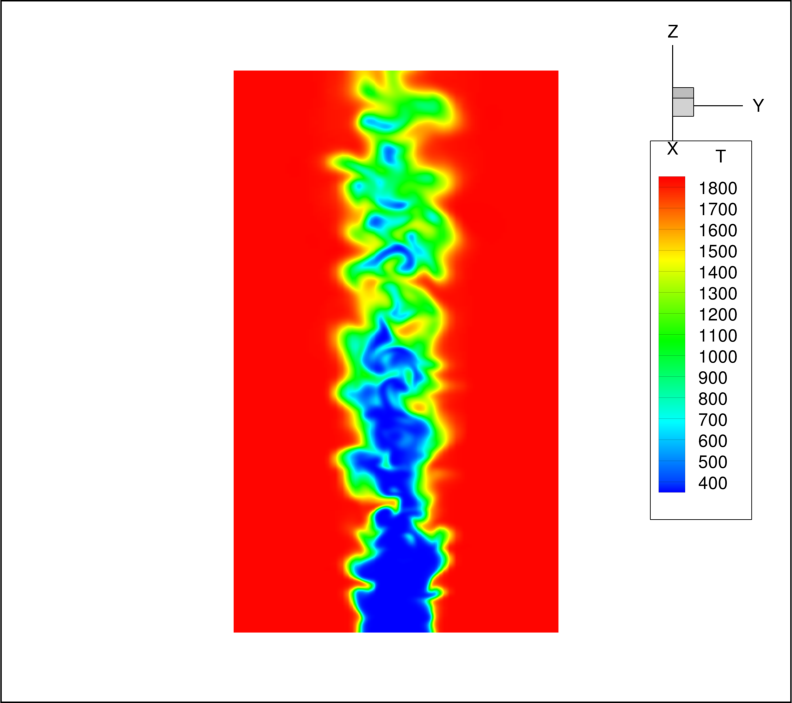
\includegraphics[width=0.21\textheight, trim=7cm 0.2cm 2cm 0.2cm,clip=true]{./figs/Flame_temp.png}}
\subfloat[\tiny{FSD at 2.0 ms} \label{fig:fsd2}]{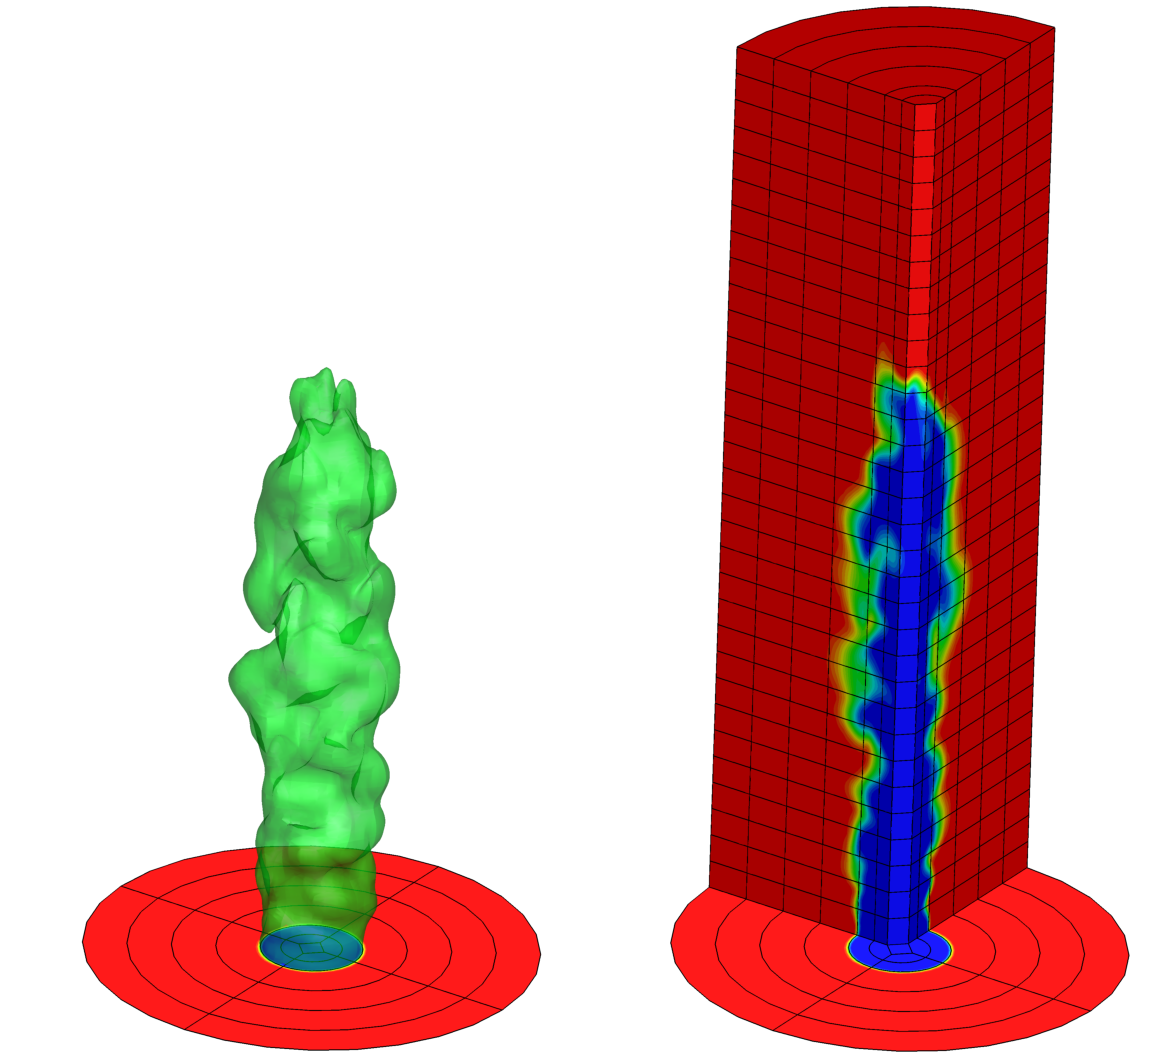
\includegraphics[width=0.3\textheight, trim=0cm 0cm 0 0cm,clip=true]{./figs/fsd2_0ms.png}}
\subfloat[\tiny{FSD at 4.25 ms} \label{fig:fsd4_25}]{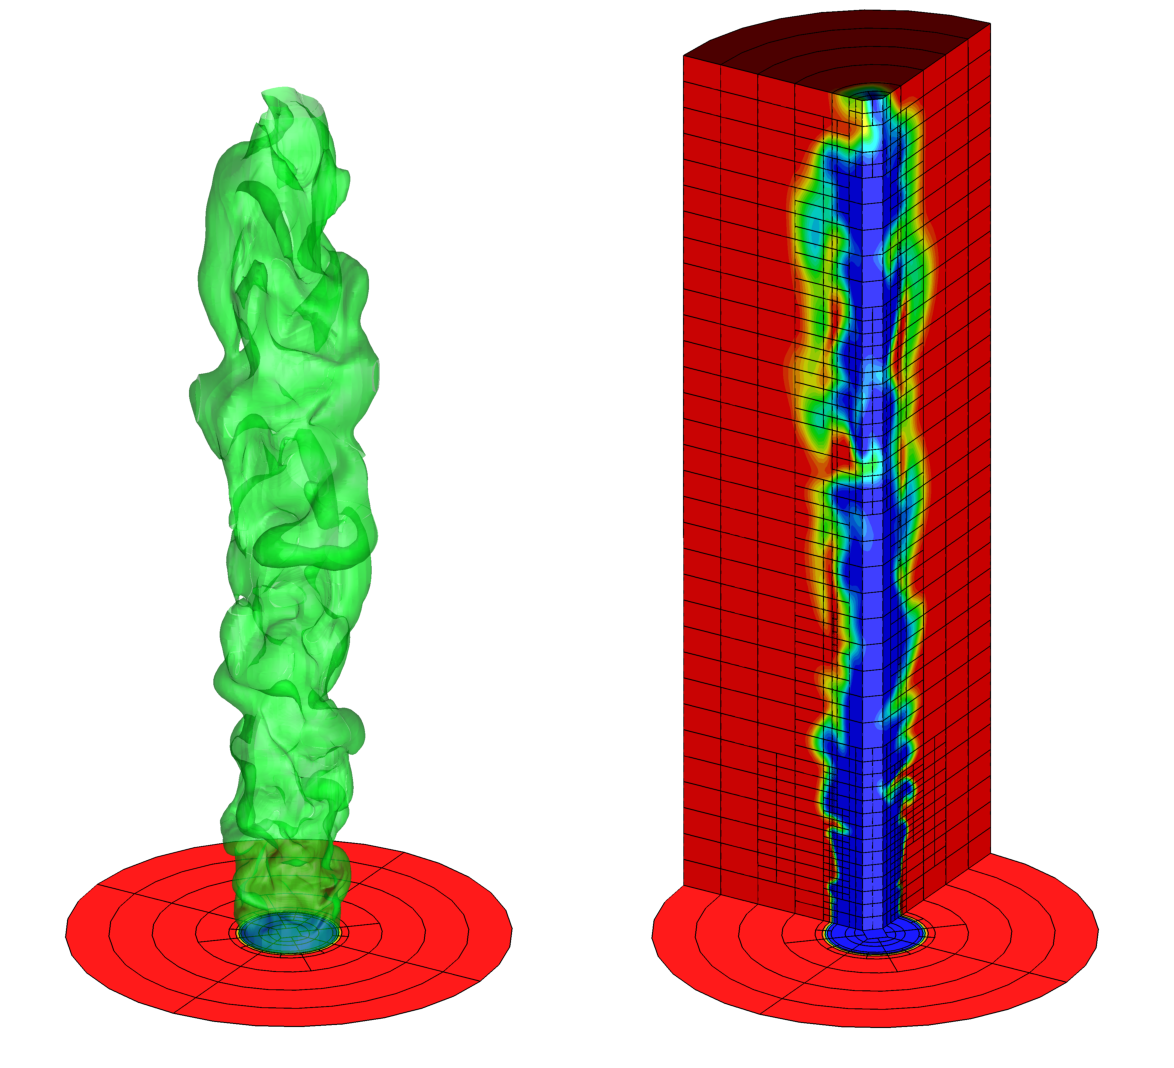
\includegraphics[width=0.3\textheight, trim=0cm 0cm 0 0cm,clip=true]{./figs/fsd4_25ms.png}}
\subfloat[\tiny{FSD at 7.0 ms } \label{fig:fsd7_0}]{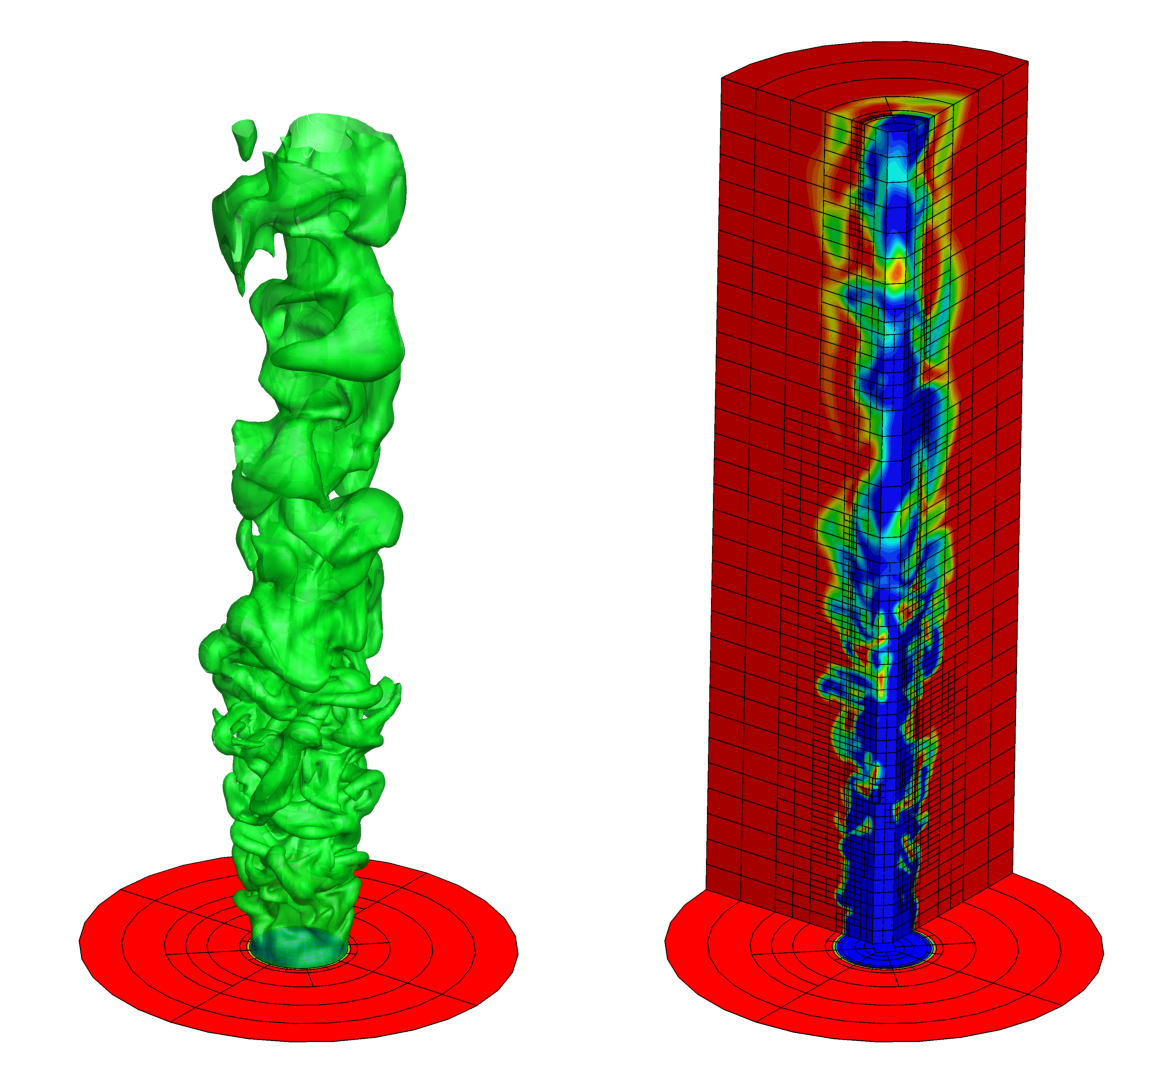
\includegraphics[width=0.3\textheight, trim=0cm 0cm 0 0cm,clip=true]{./figs/fsd7_0ms.png}}
\subfloat[\tiny{time ave $c_{O_{2}}$} \label{fig:tave}]{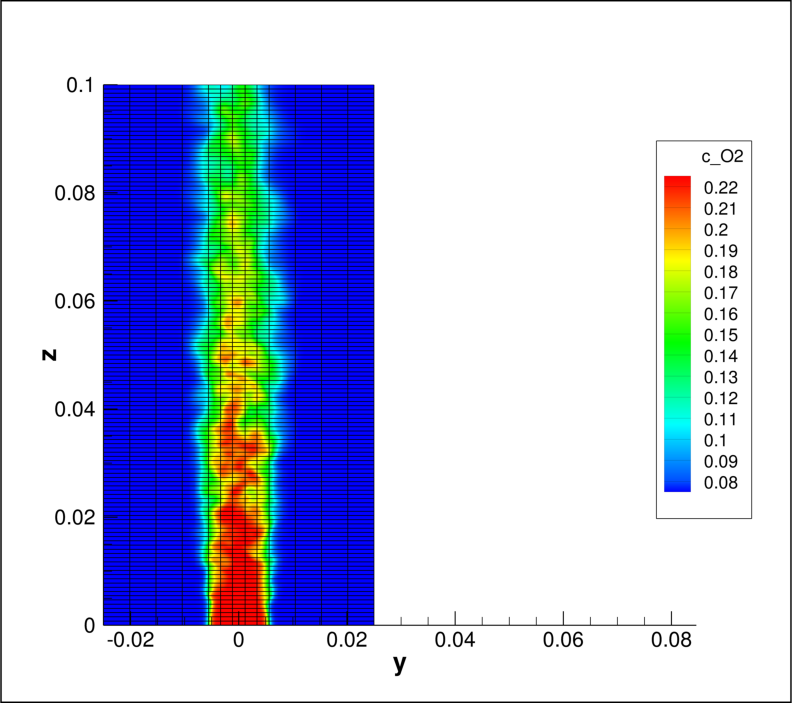
\includegraphics[width=0.25\textheight, trim=4cm 0.3cm 2cm 0.5cm,clip=true]{./figs/Time_averaged_c_O2.png}}
%\tiny{\caption{\tiny{Solution contours for Poisson problem}}}
\end{figure}

Computational costs:
\begin{itemize}
\tiny
\item (a) and (e): 800 procs, 3200 (8x8x8) blocks, ~1.64 x$10^6$ cells, no refinement, ~125x$10^3$ CPU hrs 
\item (b) 800 (8x8x8) blocks, ~410,000 cells,  no refinement
\item (c) 5595 (8x8x8) blocks, ~2.8 million cells, 3 levels of mesh refinement
\item (d) 18531 (8x8x8) blocks, ~9.5 million cells, 3 levels of mesh refinement
\end{itemize}

\end{exampleblock}
\end{minipage}


\end{frame}

%------------------------------------------------------------------------

\subsection{Adjoint runs}
\begin{frame}
\frametitle{Work on the adjoint}
\begin{minipage}[t][1\textheight]{1\textwidth}
\vspace{-20pt}
\begin{exampleblock}{Preliminary work with the discrete adjoint - shockcube problem}
\vspace{-20pt}
\tiny
\begin{figure}
\label{fig:shockedcube}
\centering
\subfloat[\tiny{$\rho.u$} \label{fig:rhoU}]
{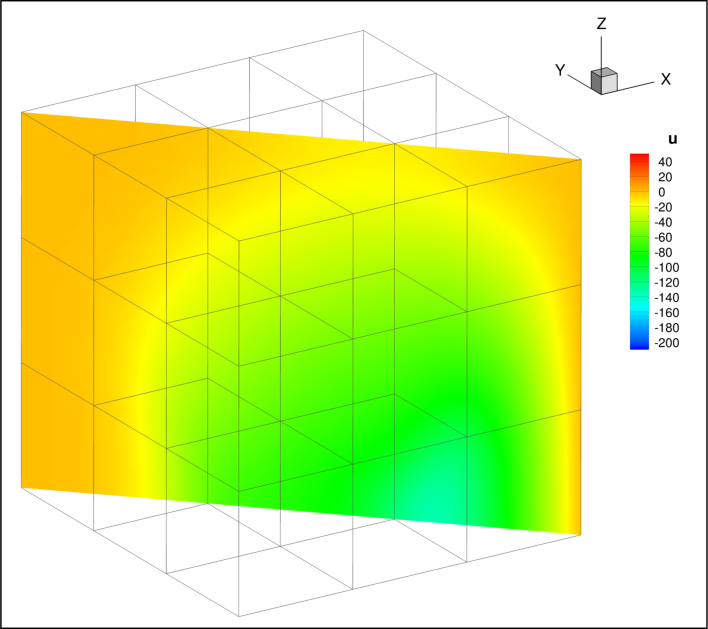
\includegraphics[width=0.65\textheight, trim=0cm 0cm 0cm 0cm,clip=true]{./figs/rhoU.png}}
\subfloat[\tiny{$\Psi_{rho.u}$} \label{fig:adjRhoU}]
{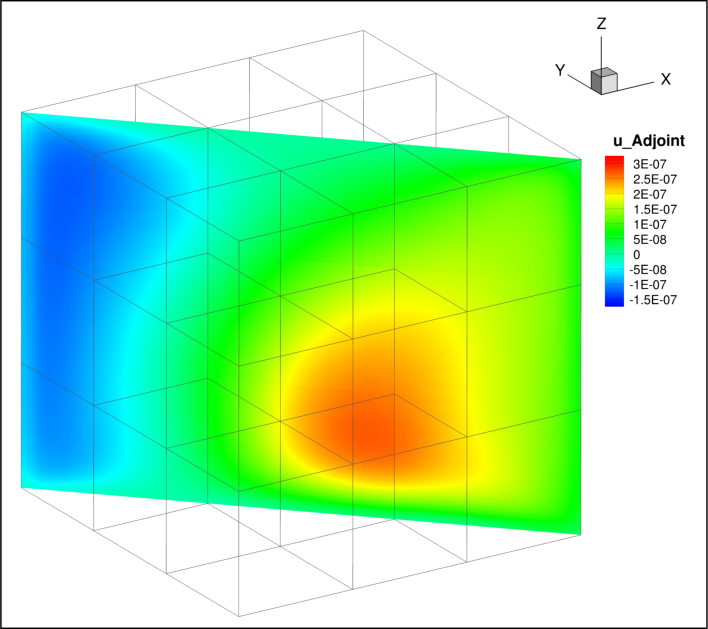
\includegraphics[width=0.65\textheight, trim=0cm 0cm 0 0cm,clip=true]{./figs/rhoU_adjoint.png}}
\end{figure}
\vspace{-10pt}
\begin{itemize}
\scriptsize
\item give the initial states, l and r: Initial conditions: $\frac{\rho_L}{\rho_R} \approx 6$. Adjoint evaluated at t = 0.035 sec.
\item how the code was modified - multiblock and multiproc for uniform blocks
\item Selected as functional the average pressure in the shockcube.

\end{itemize}

\end{exampleblock}
\end{minipage}

\end{frame}


%==========================================================================
\section[Timeline]{Timeline}

\subsection[Present]{Work done to date}
\begin{frame}%[allowframebreaks]
\frametitle{Timeline: April 2015  - January 2016}
\scriptsize

\begin{minipage}[t][1\textheight]{1\textwidth}
\vspace{-20pt}
\begin{exampleblock}{Work done to date}

\begin{tabular}{|l|c|} \hline
\multicolumn{1}{|c|}{\bf{Task}} & \multicolumn{1}{|c|}{\bf{Completion Date}} \\

\hline Literature Review & September-October 2014 \\

\hline Trelis Meshing Software & November 2014 \\

\hline CFFC Group Code Flux Jacobian Analysis & December 2014 \\

\hline Trilinos Package solution for & December 2014 \\ Poisson Problem in serial &\\and parallel configurations & \\

\hline Running a current-state LES case of a Turbulent & January 2015\\ Premixed  Methane Flame using PCM-FPI to & \\ get a threshold estimation & \\ of solution run time &\\

\hline Implementing the approximate Adjoint Derivative & March 2015 \\  to the Flux Jacobians &\\ testing on Euler Equations  &\\

\hline
\end{tabular}

\end{exampleblock}
\end{minipage}

\end{frame}


\subsection[Future]{Future work}
\begin{frame}%[allowframebreaks]
\frametitle{Future work}
\scriptsize


\begin{minipage}[t][1\textheight]{1\textwidth}
\vspace{-20pt}
\begin{exampleblock}{Projected milestones}

\begin{tabular}{|l|c|} \hline
\multicolumn{1}{|c|}{\bf{Task}} & \multicolumn{1}{|c|}{\bf{Completion Date}} \\

\hline Extension to Mesh adaptation & May 2015\\

\hline Application of Adjoint Problem to Navier Stokes  & June 2015\\

\hline Explicit Filters for High Order FVM implementation  & October 2015\\

\hline Coupling of High Order method with Adjoint-based AMR & December 2015\\

\hline CFD simulation of Cold Flow & January 2016\\

\hline CFD simulation of Laminar Non-Premixed Flame & February 2016\\

\hline CFD simulation of Laminar Diffusion Flame & February 2016\\

\hline Conference Paper II draft & April 2016\\

\hline CFD simulation of Turbulent Non-Premixed Flame & May 2016\\

\hline CFD simulation of Full Thermo-coupling & October 2016\\

\hline Thesis write-up & September 2017 \\ 

\hline

\end{tabular}

\end{exampleblock}
\end{minipage}





\end{frame}


%==========================================================================
\begin{frame}
\begin{center}
{\huge Thank You For Your Attention!} \\
\vspace*{1.5cm}
{\Large Questions?}
\end{center}
\end{frame}
%==========================================================================

\appendix
\newcounter{finalframe}
\setcounter{finalframe}{\value{framenumber}}

\begin{frame}
\frametitle{References}
\begin{thebibliography}{1} %Using the bibtex package is recoended but this should allow you do the bibliograghy ad-hoc.
\begin{tiny}
\beamertemplatetextbibitems
\bibitem{MooreLaw}
BCA Research Blog, \newblock {\url{http://blog.bcaresearch.com/wp-content/uploads/2013/10/Chart-III-8-Moores-Law-Over-199-Years-And-Going-Strong.png}}, Accessed 29-03-2015
\bibitem{Kohler}
K{\"o}hler, M., Boxx, I., Geigle, K. P., and Meier, W., \newblock Simultaneous planar measurements of soot structure and velocity fields in a turbulent lifted jet flame at 3-kHz", Applied Physics B 103 (2), 271-279, 2011  
\bibitem{AdelaideISF}
Adelaide international sooting flame (ISF) workshop, \newblock \url{http://www.adelaide.edu.au/cet/isfworkshop/data-sets/turbulent/}, Accessed 29-03-2015
\bibitem{Pope}
Yang, Y., Pope, S. B., Chen, J. H., \newblock "An LES/PDF study of a turbulent lifted ethylene jet flame in a heated coflow", 8th US National Combustion Meeting, 2013
\bibitem{Graetsch}
Gr{\"a}tsch, T., Bathe, K. J., \newblock "A posteriori error estimation techniques in practical finite element analysis", Journal of Computers and Structures 83, 235–265 , 2005 
\bibitem{Bibb}
Bibb, K., Gnoffo, P. A., Park, M. A., Jones, W. T., \newblock "Parallel, Gradient-Based Anisotropic Mesh Adaptation for Re-entry Vehicle Configurations",  AIAA/ASME Joint Thermophysics and Heat Transfer Conference, AIAA Paper 2006–3579, 2006 
\end{tiny}
\end{thebibliography}
\end{frame}
%==========================================================================

\setcounter{framenumber}{\value{finalframe}}
\end{document}




%==========================================================================